\section{Dynamic models}
\begin{slide}\slidetitle{Dynamic models}
\tableofcontents[sectionstyle=show/hide,subsectionstyle=show/shaded/hide]

\end{slide}\subsection{Dependent data}\begin{slide}
\slidetitle{Dependent data}

Huge portion of real-life data involving dependent datapoints

\vs\pause
\begin{example}[Capture-recapture]\begin{itemize}
\item capture histories
\item capture sizes
\end{itemize}\end{example}

\end{slide}\begin{slide}
\slidetitle{{\sf Eurostoxx 50}}

First four stock indices of of the financial index
{\sf Eurostoxx 50}

\centerline{\includegraphics[height=10cm,angle=270,width=7cm]{figures/Euro.eps}}

\end{slide}\begin{slide}
\slidetitle{Markov chain}

Stochastic process $(x_t)_{t\in\mathcal{T}}$
where distribution of $x_t$ given the past values $\bx_{0:(t-1)}$
only depends on $x_{t-1}$.

Homogeneity:  distribution of $x_t$ given the past constant in
$t\in\mathcal{T}$.

\vs\pause
Corresponding likelihood
$$
\ell(\theta|\bx_{0:T}) = f_0(x_0|\theta)\,\prod_{t=1}^T f(x_t|x_{t-1},\theta)
$$

\pause{\em [Homogeneity means $f$ independent of $t$]}

\end{slide}\begin{slide}
\slidetitle{Stationarity constraints}

Difference with the independent case: {\em stationarity} and {\em causality}
constraints put restrictions on the parameter space

\end{slide}\begin{slide}
\slidetitle{Stationarity processes}

\begin{definition}[Stationary stochastic process]
$(x_t)_{t\in\mathcal{T}}$ is stationary if the joint distributions of
$(x_1,\ldots,x_k)$ and $(x_{1+h},\ldots,x_{k+h})$ are the same for all $h,k$'s.\\

\pause
It is {\em second-order stationary} if, given 
the autocovariance function 
$$
\gamma_x(r,s)=\mathbb{E}[\{x_r-\mathbb{E}(x_r)\}\{x_s-\mathbb{E}(x_s)\}],
\quad r,s\in \mathcal{T}\,,
$$
then
$$
\mathbb{E}(x_t)=\mu \quad\text{and}\quad \gamma_x(r,s)=\gamma_x(r+t,s+t)\equiv\gamma_x(r-s)
$$
for all $r,s,t\in\mathcal{T}$.
\end{definition}

\end{slide}\begin{slide}
\slidetitle{Imposing or not imposing stationarity}

Bayesian inference on a non-stationary process can be [formaly] conducted

\pause
\begin{block}{Debate}
From a Bayesian point of view, to impose the {\it stationarity} condition is objectionable:\small
stationarity requirement on finite datasets artificial {\em and/or} 
datasets themselves should indicate whether the model is stationary\\ 
\normalsize
Reasons for imposing stationarity:\small
asymptotics (Bayes estimators are not necessarily convergent in
non-stationary settings) causality, identifiability and ... common practice.\normalsize
\end{block}

\end{slide}\begin{slide}
\slidetitle{Unknown stationarity constraints}

Practical difficulty: for complex models, 
stationarity constraints get quite involved to the
point of being unknown in some cases 

\end{slide}\subsection{The AR$(p)$ model}\begin{slide}
\slidetitle{The AR$(1)$ model}

Case of linear Markovian dependence on the last value
$$
x_t=\mu + \varrho (x_{t-1} -\mu) + \epsilon_t \,,\epsilon_t
\stackrel{\text{i.i.d.}}{\sim} \mathscr{N}(0,\sigma^2)
$$

\vs\pause
If $|\varrho|<1$, $(x_t)_{t\in\mathbb{Z}}$ can be written as
$$
x_t=\mu + \sum_{j=0}^\infty \varrho^j \epsilon_{t-j}
$$
and this is a stationary representation.

\end{slide}\begin{slide}
\slidetitle{Stationary but...}

If $|\varrho|>1$, alternative stationary representation
$$
x_t=\mu-\sum_{j=1}^\infty \varrho^{-j} \epsilon_{t+j}\,.
$$

\vs\pause
This stationary solution is criticized as 
artificial because $x_t$ is correlated with {\em
future} white noises $(\epsilon_t)_{s>t}$, unlike the case when $|\varrho|<1$.

{\em Non-causal} representation...

\end{slide}\begin{slide}
\slidetitle{Standard constraint}

\copyright~Customary to restrict AR$(1)$
processes to the case $|\varrho|<1$ 

\pause \vs 
Thus use of a uniform prior on $[-1,1]$ for $\varrho$

\vs\pause\small
Exclusion of the case $|\varrho|=1$ that leads to a random walk
because the process is then a random walk {\em [no stationary solution]}
\normalsize

\end{slide}\begin{slide}
\slidetitle{The AR$(p)$ model}

Conditional model
\[
x_t|x_{t-1},\ldots \sim
\CN\left(\mu + \sum_{i=1}^p \varrho_i (x_{t-i}-\mu),\sigma^2\right)
\]

\pause
\begin{itemize}
\item Generalisation of AR$(1)$
\item Among the most commonly used models in dynamic settings
\item More challenging than the static models (stationarity constraints)
\item Different models depending on the processing of the starting value $x_0$
\end{itemize}

\end{slide}\begin{slide}
\slidetitle{Stationarity+causality}

Stationarity constraints in the prior as a restriction
on the values of $\theta$. 

\begin{theorem}
{\RawSienna{AR$(p)$ model second-order stationary and causal 
{\Sepia{\sf iff}} the roots of the polynomial
$$
\CP(x) = 1 - \sum_{i=1}^p \varrho_i x^i
$$
are all outside the unit circle}}
\end{theorem}

\end{slide}\begin{slide}
\slidetitle{Initial conditions}

Unobserved initial values can be processed in various ways
\begin{enumerate} 
\item All $\bx_{-i}$'s $(i>0)$ set equal to $\mu$, for computational convenience 
\pause
\item Under stationarity and causality constraints, 
$(x_t)_{t\in\mathbb{Z}}$ has a stationary distribution: Assume $\bx_{-p:-1}$ distributed from
stationary $\mathscr{N}_p(\mu{\mathbf 1}_p,\mathbf{A})$ distribution\\ Corresponding
marginal likelihood
\footnotesize\begin{align*}
\int \sigma^{-T} \prod_{t=0}^T &\exp\left\{\frac{-1}{2\sigma^2}\left(x_t-\mu - \sum_{i=1}^p \varrho_i (x_{t-i}-\mu)
\right)^2 \right\}\\
&f(\bx_{-p:-1}|\mu,\mathbf{A})\,\text{d}\bx_{-p:-1}\,,
\end{align*}\normalsize
\end{enumerate}

\end{slide}\begin{slide}
\slidetitle{Initial conditions (cont'd)}

\begin{enumerate}\setcounter{enumi}{2}
\item Condition instead on the initial {\em observed} values $\bx_{0:(p-1)}$\small
\begin{eqnarray*}
 && \ell^c(\mu,\varrho_1,\ldots,\varrho_p,\sigma|\bx_{p:T},\bx_{0:(p-1)}) \propto \\
 && \qquad \sigma^{-T} \prod_{t=p}^T \exp\left\{-\left(x_t-\mu - \sum_{i=1}^p \varrho_i (x_{t-i}-\mu) \right)^2 \big/ 2\sigma^2 \right\}\,. \normalsize
\end{eqnarray*}
\end{enumerate}


\end{slide}\begin{slide}
\slidetitle{Prior selection}

For AR$(1)$ model, Jeffreys' prior associated with the stationary representation is
$$
\pi_1^J(\mu,\sigma^2,\varrho) \propto \frac{1}{\sigma^2} \frac{1}{\sqrt{1-\varrho^2}} \,.
$$

\pause Extension to higher orders quite complicated ($\varrho$ part)!

\vs\pause Natural conjugate prior for
$\theta=(\mu,\varrho_1,\ldots,\allowbreak \varrho_p,\allowbreak \sigma^2)$ :\\
normal distribution on $(\mu,\varrho_1,\ldots,\varrho_p)$ 
and inverse gamma distribution on $\sigma^2$

\pause... and for constrained $\varrho$'s?

\end{slide}\begin{slide}
\slidetitle{Stationarity constraints}

Under stationarity constraints, complex parameter space: each value of $\varrho$ needs
to be checked for roots of corresponding polynomial with modulus less than $1$

\vs\pause
E.g., for an AR$(2)$ process with autoregressive polynomial
$\mathcal{P}(u)=1-\varrho_1u-\varrho_2u^2$, constraint is
$$
\varrho_1+\varrho_2<1, \quad \varrho_1-\varrho_2<1 \quad\text{and}\quad |\varrho_2|<1\,.
$$
\begin{flushright}
\hyperlink{Rootpara}{\beamergotobutton{Skip Durbin forward}}
\end{flushright}

\end{slide}\begin{slide}[label=DLrepa]
\slidetitle{A first useful reparameterisation}

{\RedViolet{\em Durbin--Levinson recursion}} proposes a {\em reparametrisation}  
from the parameters $\varrho_i$ to the {\em partial autocorrelations}
$$
  \psi_i \in [-1,1]
$$
which allow for a uniform prior on the hypercube.

\pause
Partial autocorrelation defined as
\begin{align*}
\psi_i = \text{corr}&\left(x_t-\mathbb{E}[x_t|x_{t+1},\ldots,x_{t+i-1}],\right.\\
&\left.x_{t+i}-\mathbb{E}[x_{t+1}|x_{t+1},\ldots,x_{t+i-1}] \right)
\end{align*}
{\em [see also Yule-Walker equations]}

\end{slide}\begin{slide}
\slidetitle{Durbin--Levinson recursion}

\begin{block}{Transform}
{\sffamily
\begin{enumerate}
\item {\sf Define  $\varphi^{ii} = \psi_i$  and
$\varphi^{ij} = \varphi^{(i-1)j} - \psi_i \varphi^{(i-1)(i-j)}$,
for $i > 1$  and  $j=1,\cdots,i-1$ .}

\item {\sf Take $\varrho_i = \varphi^{pi}$ for $i=1,\cdots,p$.}
\end{enumerate}}
\end{block}

\end{slide}\begin{slide}
\slidetitle{Stationarity \&\ priors}

For AR$(1)$ model, Jeffreys' prior associated with the stationary representation is 
$$
\pi_1^J(\mu,\sigma^2,\varrho) \propto \frac{1}{\sigma^2} \frac{1}{\sqrt{1-\varrho^2}} \,.
$$

Within the non-stationary region $|\varrho| > 1$, Jeffreys' prior is 
$$
\pi_2^J(\mu,\sigma^2,\varrho) \propto \frac{1}{\sigma^2} 
\frac{1}{\sqrt{|1-\varrho^2|}}
\sqrt{ \left| 1 - \frac{1-\varrho^{2T}}{T(1-\varrho^2)} \right| }\,.
$$

\centerline{\MidnightBlue{\fbox{\sf The dominant part of the prior is the non-stationary region!}}}

\end{slide}\begin{slide}
\slidetitle{Alternative prior}

The reference prior $\pi_1^J$ is only defined when the stationary constraint holds. 

{\BurntOrange{Idea}} Symmetrise to the region $|\varrho| > 1$
$$
\pi^B(\mu,\sigma^2,\varrho) \propto \frac{1}{\sigma^2} 
\begin{cases} 1/\sqrt{1-\varrho^2} & \hbox{if }|\varrho| < 1,\cr
        1/|\varrho| \sqrt{\varrho^2-1} & \hbox{if }|\varrho| > 1,\cr\end{cases} \,,
$$

\includegraphics[height=10cm,width=4cm,angle=270]{figures/statiozone.ps}

\end{slide}\begin{slide}
\slidetitle{MCMC consequences}

When devising an MCMC algorithm, use the Durbin-Levinson recursion to end up with
single normal simulations of the $\psi_i$'s since the $\varrho_j$'s are linear
functions of the $\psi_i$'s

\end{slide}\begin{slide}[label=Rootpara]
\slidetitle{Root parameterisation}

\hyperlink{DLrepa}{\beamerreturnbutton{Skip Durbin back}}Lag polynomial representation 
$$
\left(\hbox{Id} - \sum_{i=1}^p \varrho_i B^i\right)\,x_t = \epsilon_t
$$
with (inverse) roots
$$
\prod_{i=1}^p \left( \hbox{Id} - \lambda_i B\right) \,x_t = \epsilon_t
$$

\vs\pause
Closed form expression of the likelihood as a function of the (inverse) roots

\end{slide}\begin{slide}
\slidetitle{Uniform prior under stationarity} 

\BurntOrange{Stationarity} The $\lambda_i$'s are within the unit circle 
if in $\mathbb{C}$ [complex numbers] and within $[-1,1]$ if in $\mathbb{R}$ 
[real numbers]

\vs\pause
Naturally associated with a flat prior on either the unit circle or $[-1,1]$
$$
\frac{1}{\lfloor k/2 \rfloor+1}
\,\prod_{\lambda_i\in{\mathbb R}} \frac{1}{2}{\mathbb I}_{|\lambda_i|<1}
\,\prod_{\lambda_i\not\in{\mathbb R}} \frac{1}{\pi}{\mathbb I}_{|\lambda_i|<1}
$$
where $\lfloor k/2 \rfloor+1$ number of possible cases

\vs\pause\begin{itemize}
\item[$\lightning$] Term $\lfloor k/2 \rfloor+1$ is important 
for reversible jump applications
\end{itemize}

\end{slide}\begin{slide}
\slidetitle{MCMC consequences}

In a Gibbs sampler, each $\lambda_{i^*}$ can be simulated conditionaly on the others since
$$
\prod_{i=1}^p \left( \hbox{Id} - \lambda_i B\right) \,x_t =
y_t - \lambda_{i^*} y_{t-1} = \epsilon_t
$$
where
$$
Y_t = \prod_{i\ne i^*} \left( \hbox{Id} - \lambda_i B\right) \,x_t
$$

\end{slide}\begin{slide}
\slidetitle{Metropolis-Hastings implementation}

\begin{enumerate}
\item use the prior $\pi$ itself as a proposal on
the (inverse) roots of $\mathcal{P}$, selecting one
or several roots of $\mathcal{P}$ to be simulated from $\pi$;
\item acceptance ratio is likelihood ratio
\item need to watch out for real/complex dichotomy
\end{enumerate}

\end{slide}\begin{slide}
\slidetitle{A [paradoxical] reversible jump implementation}

\small\begin{itemize}
\item Define ``model" $\mathfrak{M}_{2k}$ $(0\le k\le \lfloor
p/2 \rfloor)$ as corresponding to a number $2k$ of complex roots
$o\le k\le \lfloor p/2 \rfloor)$

\item Moving from model $\mathfrak{M}_{2k}$ to model $\mathfrak{M}_{2k+2}$ means that
two real roots have been replaced by two conjugate complex roots.

\item Propose jump from $\mathfrak{M}_{2k}$ to 
$\mathfrak{M}_{2k+2}$ with probability $1/2$ and from 
$\mathfrak{M}_{2k}$ to $\mathfrak{M}_{2k-2}$ with probability
$1/2$ {\em [boundary exceptions]}

\item accept move from $\mathfrak{M}_{2k}$ to $\mathfrak{M}_{2k+\,\text{or}\,-2}$
with probability
$$
\frac{\ell^c(\mu,\varrho_1^\star,\ldots,\varrho_p^\star,\sigma|\bx_{p:T},\bx_{0:(p-1)})}
     {\ell^c(\mu,\varrho_1,\ldots,\varrho_p,\sigma|\bx_{p:T},\bx_{0:(p-1)})}\,\wedge\,1\,,
$$
\end{itemize}
\normalsize
\end{slide}\begin{slide}
\slidetitle{Checking your code}

Try with no data and recover the prior

\only<1>{\includegraphics[height=2cm,angle=270,width=8cm,draft=T]{figures/checkin.eps}}

\end{slide}\begin{slide}
\slidetitle{Checking your code}

Try with no data and recover the prior

\only<1>{\includegraphics[height=2cm,angle=270,width=8cm,draft=T]{figures/chicken.eps}}

\end{slide}\begin{slide}
\slidetitle{Order estimation}

Typical setting for model choice: determine order $p$ of $AR(p)$ model

Roots [may] change drastically from one $p$ to the other.

No difficulty from the previous perspective: recycle above reversible jump
algorithm

\end{slide}\begin{slide}
\slidetitle{AR(?) reversible jump algorithm}

Use (purely birth-and-death) proposals based on the uniform prior
\def\too{$\rightarrow$}
\begin{itemize}
\item {\Sepia{\sf k  \too\ k+1}}  {\BurntOrange{\sf \quad[Creation of real root]}}
\item {\Sepia{\sf k  \too\ k+2}}  {\BurntOrange{\sf \quad[Creation of complex root]}}
\item {\Sepia{\sf k  \too\ k-1}}  {\BurntOrange{\sf \quad[Deletion of real root]}}
\item {\Sepia{\sf k  \too\ k-2}}  {\BurntOrange{\sf \quad[Deletion of complex root]}}
\end{itemize}

\end{slide}\begin{slide}
\slidetitle{Reversible jump output}

\includegraphics[width=5cm,height=10cm,angle=270]{figures/plain.ps}

\footnotesize
$AR(3)$ simulated dataset of 530 points {\em (upper left)} 
with true parameters $\alpha_i$ $(-0.1,0.3,-0.4)$ and $\sigma=1$.
{\em First histogram} associated with $p$, following
histograms with the $\alpha_i$'s, for
different values of $p$, and of $\sigma^2$. {\em Final graph:} scatterplot
of the complex roots. {\em One before last:} evolution of $\alpha_1,\alpha_2,\alpha_3$.
\normalsize

\end{slide}\subsection{The MA$(q)$ model}\begin{slide}
\slidetitle{The MA$(q)$ model}

Alternative type of time series
\[
  x_t = \mu +\epsilon_t - \sum_{j=1}^q \vartheta_j \epsilon_{t-j}
    \,,\quad \epsilon_t\sim\CN(0,\sigma^2)
\]

Stationary but, for identifiability considerations, the polynomial
$$
\CQ(x) = 1 - \sum_{j=1}^q \vartheta_j x^j
$$
must have all its roots outside the unit circle.

\end{slide}\begin{slide}
\slidetitle{Identifiability}

\debut For the MA$(1)$ model, $x_t
= \mu +\epsilon_t - \vartheta_1\epsilon_{t-1}$, 
$$
{\varm}(x_t)=(1+\vartheta_1^2)\sigma^2
$$
can also be written 
$$
x_t = \mu + \tilde \epsilon_{t-1} - \frac{1}{\vartheta_1} \tilde
\epsilon_{t},\,\quad
\tilde\epsilon\sim\CN(0,\vartheta_1^2\sigma^2)\,,
$$
Both pairs $(\vartheta_1,\sigma)$ \&\
$(1/\vartheta_1,\vartheta_1\sigma)$ lead to 
alternative representations of the {\em same} model.  \fin

\end{slide}\begin{slide}
\slidetitle{Properties of MA models}

\begin{itemize}
\item Non-Markovian model (but special case of hidden Markov)
\item Autocovariance $\gamma_x(s)$ is null for $|s|>q$
\end{itemize}

\end{slide}\begin{slide}
\slidetitle{Representations}

$\bx_{1:T}$ is a normal random variable with constant mean $\mu
$ and covariance matrix\small
$$
\Sigma = \left(
\begin{matrix} \sigma^2 &\gamma_1 &\gamma_2 &\ldots &\gamma_q &0 &\ldots &0
&0\cr
         \gamma_1 &\sigma^2 &\gamma_1 &\ldots &\gamma_{q-1} &\gamma_q
&\ldots &0 &0\cr
	 & & &\ddots & & & & &\cr
	 0 &0 &0 &\ldots &0 &0 &\ldots &\gamma_1 &\sigma^2\cr \end{matrix}
\right) \,,
$$\normalsize
with $(|s|\le q)$
\[
  \gamma_s = \sigma^2 \sum_{i=0}^{q-|s|} \vartheta_i \vartheta_{i+|s|}
\]

Not manageable in practice {\em [large T's]}

\end{slide}\begin{slide}
\slidetitle{Representations (contd.)}

Conditional on past $(\epsilon_0,\ldots, \epsilon_{-q+1})$,
\small\begin{eqnarray*}
&&L(\mu,\vartheta_1,\ldots,\vartheta_q,\sigma|x_{1:T},\epsilon_0,\ldots,
\epsilon_{-q+1}) \propto \\
&&\qquad \sigma^{-T} \prod_{t=1}^T
	 \exp\left\{-\left(x_t-\mu+ \sum_{j=1}^q \vartheta_j
	 \hat \epsilon_{t-j} \right)^2
\big/ 2\sigma^2 \right\} \,, 
\end{eqnarray*}
\normalsize where $(t>0)$
\[
\hat \epsilon_t = x_t -\mu + \sum_{j=1}^q \vartheta_j \hat\epsilon_{t-j},\
\hat \epsilon_{0}=\epsilon_0,\ \ldots,\ \hat \epsilon_{1-q}=\epsilon_{1-q}
\]

Recursive definition of the likelihood, still costly ${\mathrm O}(T\times q)$

\end{slide}\begin{slide}
\slidetitle{Recycling the AR algorithm}

Same algorithm as in the AR$(p)$ case when modifying the likelihood

\vs\pause
Simulation of the past noises $\boldsymbol{\epsilon}_{-i}$
$(i=1,\ldots,q)$ done via a Metropolis-Hastings step with target
$$
f(\epsilon_0,\ldots,\epsilon_{-q+1}|\bx_{1:T},\mu,\sigma,\boldsymbol{\vartheta}) \propto
\prod_{i=-q+1}^0 e^{-\epsilon_i^2/2\sigma^2}\,
\prod_{t=1}^T e^{-\widehat\epsilon_t^2/2\sigma^2}\,,
$$

\end{slide}\begin{slide}
\slidetitle{Representations (contd.)}

Encompassing approach for general time series models

\vs {\RedViolet{\sf State-space representation}}
\begin{eqnarray}
{\mathbf x_t} &=& G {\mathbf y}_t + \boldsymbol{\varepsilon}_t\,,
\label{eq:staspa.obs}\\
{\mathbf y}_{t+1} &=& F {\mathbf y}_t + {\mathbf \xi}_t\,,
\label{eq:staspa.stat}
\end{eqnarray}

(\ref{eq:staspa.obs}) is the {\it observation equation} and
(\ref{eq:staspa.stat}) is the {\it state equation}

\vs\pause
\begin{block}{Note}
As seen below, this is a special case of hidden Markov model
\end{block}

\end{slide}\begin{slide}
\slidetitle{MA$(q)$ state-space representation}

For the MA$(q)$ model, take
\[
{\mathbf y}_t = ( \epsilon_{t-q},\ldots,
\epsilon_{t-1}, \allowbreak\epsilon_{t} )^\prime
\]
and then
\small\begin{eqnarray*}
{\mathbf y}_{t+1} &=& \left( \begin{matrix} 0 &1 &0 &\ldots &0\cr
				     0 &0 &1 &\ldots &0\cr
                                       &  &  &\ldots & \cr
				     0 &0 &0 &\ldots &1\cr
				     0 &0 &0 &\ldots &0\cr
		\end{matrix} \right) {\mathbf y}_t 
	+ \epsilon_{t+1} \left( \begin{matrix}
				0\cr 0\cr \vdots\cr 0\cr 1\cr
				\end{matrix} \right) \\
x_t &=& \mu - \left( \begin{matrix}\vartheta_q &\vartheta_{q-1} &\ldots
&\vartheta_1 &-1\end{matrix}\right) {\mathbf y}_t \,.
\end{eqnarray*}\normalsize

\end{slide}\begin{slide}
\slidetitle{MA$(q)$ state-space representation (cont'd)}

\debut
For the MA$(1)$ model, observation equation 
$$
  x_t = (\begin{matrix}1 &0\end{matrix}) {\mathbf y}_t
$$
with 
$$
  {\mathbf y}_t = (\begin{matrix}y_{1t} &y_{2t}\end{matrix})^\prime
$$
directed by the state equation
$$
  {\mathbf y}_{t+1} = \left( \begin{matrix} 0 &1\cr 0 &0\end{matrix}\right) {\mathbf y}_t
  + \epsilon_{t+1} \left( \begin{matrix} 1 \cr \vartheta_1\cr\end{matrix}\right)\,.
$$
\fin

\end{slide}\begin{slide}
\slidetitle{ARMA extension}

ARMA$(p,q)$ model
\[\BurntOrange{
  x_t - \sum_{i=1}^p \varrho_i x_{t-1} = \mu +\epsilon_t 
  - \sum_{j=1}^q \vartheta_j \epsilon_{t-j}
  \,,\quad \epsilon_t\sim\CN(0,\sigma^2)
}\]

Identical stationarity and identifiability conditions for both groups\\
$(\varrho_1,\ldots,\varrho_p)$ and $(\vartheta_1,\ldots,\vartheta_q)$

\end{slide}\begin{slide}
\slidetitle{Reparameterisation}
Identical root representations
\small{$$
\prod_{i=1}^p (\hbox{Id} - \lambda_i B) x_t =
\prod_{i=1}^q (\hbox{Id} - \eta_i B) \epsilon_t
$$}
\pause
State-space representation
$$
 \bx_t = x_t = \mu - \left( \begin{matrix} \vartheta_{r-1} &\vartheta_{r-2}
 &\ldots &\vartheta_1 &-1\end{matrix}\right) {\mathbf y}_t
$$
and
\footnotesize
$$
{\mathbf y}_{t+1} =  \left( \begin{matrix}
    0 &1 &0 &\ldots &0\cr
    0 &0 &1 &\ldots &0\cr
    &  &  &\ldots & \cr
    0 &0 &0 &\ldots &1\cr
    \varrho_r &\varrho_{r-1} &\varrho_{r-2} &\ldots &\varrho_1\cr
        \end{matrix} \right) {\mathbf y}_t + \epsilon_{t+1} \left( \begin{matrix}
                0\cr 0\cr \vdots\cr 0\cr 1\cr \end{matrix} \right) \,,
$$\normalsize
under the convention that
$\varrho_m=0$ if $m>p$ and $\vartheta_m=0$ if $m>q$.

\end{slide}\begin{slide}
\slidetitle{Bayesian approximation}

Quasi-identical MCMC implementation:
\colorbox{LightGrey}{\makebox[0.9\textwidth][c]{\parbox{0.85\textwidth}{{\sf
\Brown{
\begin{enumerate}
\item Simulate $(\varrho_1,\ldots,\varrho_p)$ conditional on $(\vartheta_1,\ldots,\vartheta_q)$ and $\mu$
\item Simulate $(\vartheta_1,\ldots,\vartheta_q)$ conditional on $(\varrho_1,\ldots,\varrho_p)$ and $\mu$
\item Simulate $(\mu,\sigma)$ conditional on $(\varrho_1,\ldots,\varrho_p)$ and $(\vartheta_1,\ldots,\vartheta_q)$
\end{enumerate}
}}}}}

\vs\pause
\copyright~Code can be recycled almost as is!

\end{slide}
\subsection{Hidden Markov models}
\begin{slide}\slidetitle{Hidden Markov models}

Generalisation both of a mixture and of a state space model.

\pause\debut
Extension of a {\em mixture} model with Markov dependence
$$
\Brown{
x_t|z,x_j\; j\ne t \; \sim \CN(\mu_{z_t},\sigma_{z_t}^2), \qquad
P(z_t=u|z_j\;, j<t) = p_{z_{t-1}u}, 
}
$$
$(u=1,\ldots,k)$
\fin

\pause\begin{itemize}
\item[$\lightning$] Label switching also strikes in this model!
\end{itemize}

\end{slide}\begin{slide}
\slidetitle{Generic dependence graph}

\begin{figure}[h]
  \setlength{\unitlength}{1mm}
\begin{center}
\begin{picture}(66,34)
\put(0,6){\makebox(0,0)[l]{$\cdots$}}
\put(6,6){\vector(1,0){10}}
\put(22,6){\circle{11}}
\put(28,6){\vector(1,0){10}}
\put(44,6){\circle{11}}
\put(50,6){\vector(1,0){10}}
\put(62,6){\makebox(0,0)[l]{$\cdots$}}
\put(22,12){\vector(0,1){10}}
\put(22,28){\circle{11}}
\put(44,12){\vector(0,1){10}}
\put(44,28){\circle{11}}
\put(22,6){\makebox(0,0){$y_t$}}
\put(44,6){\makebox(0,0){$y_{t+1}$}}
\put(22,28){\makebox(0,0){$x_t$}}
\put(44,28){\makebox(0,0){$x_{t+1}$}}
\end{picture}
\end{center}
\end{figure}

$$
(x_t,y_t) | \mathbf{x}_{0:(t-1)},\mathbf{y}_{0:(t-1)} \sim f(y_t|y_{t-1})\,f(x_t|y_t)
$$

\end{slide}\begin{slide}
\slidetitle{Definition}

Observable series $\{\mathbf{x}_t\}_{t\ge1}$ associated with a second process
$\{y_t\}_{t\ge1}$, with a finite set of $N$ possible values such that
\begin{enumerate}
\renewcommand{\theenumi}{\arabic{enumi}.}
\item indicators $Y_t$ have an homogeneous \RedOrange{{\bf Markov dynamic}}
$$\BrickRed{
    p(y_t | \by_{1:t-1}) = p(y_t | y_{t-1}) = \BP_{y_{t-1}y_t}
}$$
where $\by_{1:t-1}$ denotes  the sequence $\{y_1, y_2, \ldots,
y_{t-1}\}$.
\item Observables $x_t$ are independent conditionally on the indicators $y_t$
$$\BrickRed{
    p(\bx_{1:T} | \by_{1:T}) = \prod_{t=1}^{T} p(x_{t} | y_{t})
}$$
\end{enumerate}

\end{slide}\begin{slide}
\slidetitle{{\sf Dnadataset}}

DNA sequence {\em [made of A, C, G, and T's]} corresponding to a complete HIV
genome where A, C, G, and T have been recoded as $1,...,4$.\\


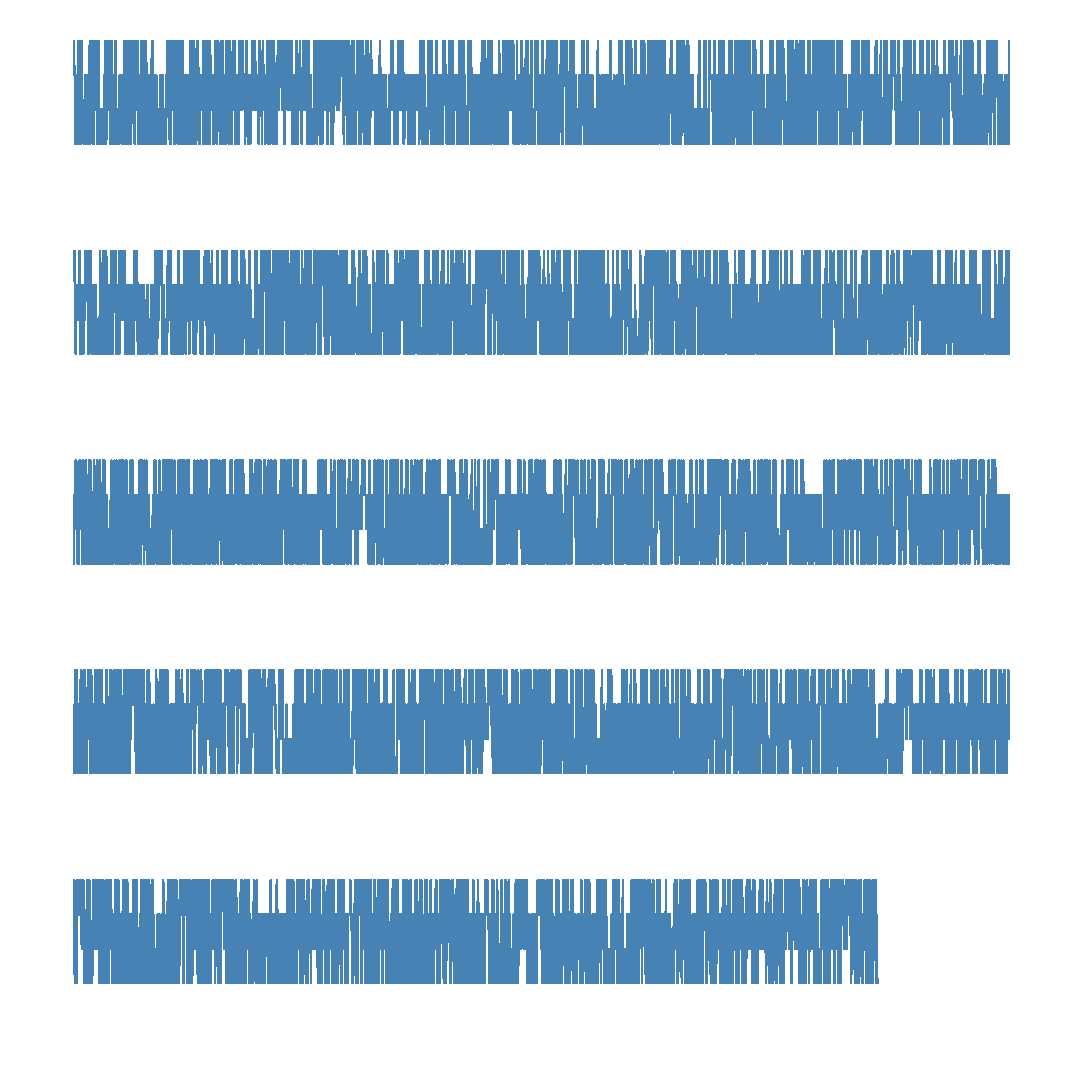
\includegraphics[height=3cm,width=\textwidth]{figures/dna.eps}

\pause
Possible modeling by a two-state hidden Markov model with 
$$
\mathscr{Y}=\{1,2\} \quad\text{and}\quad \mathscr{X}=\{1,2,3,4\}
$$

\end{slide}\begin{slide}
\slidetitle{Parameterization}

\begin{itemize}
\item For the  Markov bit, \RedViolet{{\em transition matrix}}
$$
\BP = [p_{ij}]\quad\hbox{ where }\quad\sum_{j=1}^{N} p_{ij} = 1
$$
and
\RedViolet{{\em initial  distribution}} 
$$
\varrho = \varrho \BP
$$
  
\item for the observables, 
$$\Brown{
f_i(x_t) = p(x_{t} | y_{t} = i) = f(x_t|\theta_i)
}$$
usually within the same parametrized class of distributions.
\end{itemize}

\end{slide}\begin{slide}
\slidetitle{Finite case}

When both hidden and observed chains are
finite, with $\mathscr{Y}=\{1,\ldots,\kappa\}$ and
$\mathscr{X}=\{1,\ldots,k\}$, parameter
$\theta$ made up of $p$ probability vectors
$\mathbf{q}^1=(q^1_1,\ldots\allowbreak,q^1_k),\ldots\allowbreak,
\mathbf{q}^\kappa=(q^\kappa_1,\ldots\allowbreak,q^\kappa_k)$\\

\pause
Joint distribution of $(x_t,y_t)_{0\le t\le T}$ 
$$
\varrho_{y_0}\,q^{y_0}_{x_0}\,\prod_{t=1}^T\, p_{y_{t-1}y_t}\, q^{y_t}_{x_t}\,,
$$

\end{slide}\begin{slide}
\slidetitle{Bayesian inference in the finite case}

Posterior of $(\theta,\BP)$ given $(x_t,y_t)_t$ factorizes as
$$
\pi(\theta,\BP)\,\varrho_{y_0}\,\prod_{i=1}^\kappa\,\prod_{j=1}^k (q^i_j)^{n_{ij}}
\times \prod_{i=1}^\kappa\,\prod_{j=1}^p p_{ij}^{m_{ij}}\,,
$$
where $n_{ij}$ $\#$ of visits to state $j$ by the $x_t$'s when
the corresponding $y_t$'s are equal to $i$ 
and $m_{ij}$ $\#$ of
transitions from state $i$ to state $j$ on the hidden chain
$(y_t)_{t\in\mathbb{N}}$

\vs\pause Under a flat prior on $p_{ij}$'s and
$q^i_j$'s, posterior distributions are [almost] Dirichlet
{\em [initial distribution side effect]}

\end{slide}\begin{slide}
\slidetitle{MCMC implementation}

\small
\begin{block}{Finite State HMM Gibbs Sampler}
\begin{itemize}
\item[]  {\sffamily Initialization:}
\begin{enumerate}
\item Generate random values of the $p_{ij}$'s and of the $q^i_j$'s
\item Generate the hidden Markov chain $(y_t)_{0\le t\le T}$ by $(i=1,2)$
$$
\mathbb{P}(y_t=i) \propto \begin{cases}
    p_{ii}\,q^i_{x_0}       &\text{if } t=0\,,\\
    p_{y_{t-1}i}\,q^i_{x_t}     &\text{if } t>0\,,
    \end{cases}
$$
and compute the corresponding sufficient statistics
\end{enumerate}
\end{itemize}
\end{block}\normalsize

\end{slide}\begin{slide}
\slidetitle{MCMC implementation (cont'd)}

\small
\begin{block}{Finite State HMM Gibbs Sampler}
\begin{itemize}
\item[]  {\sffamily Iteration $m$ $(m\ge 1)$:}
\begin{enumerate}
\item Generate
\begin{align*}
(p_{i1},\ldots,p_{i\kappa}) &\sim \mathscr{D}(1+n_{i1},\ldots,1+n_{i\kappa})\nonumber\\
(q^i_1,\ldots,q^i_k) &\sim \mathscr{D}(1+m_{i1},\ldots,1+m_{ik})\nonumber
\end{align*}
and correct for missing initial probability by a MH step with
acceptance probability $\varrho^\prime_{y_0}/\varrho_{y_0}$
\item Generate successively each $y_t$ $(0\le t\le T)$ by
$$
\mathbb{P}(y_t=i|x_t,y_{t-1},y_{t+1}) \propto \begin{cases}
    p_{ii}\,q^i_{x_1}\,p_{i y_1}            &\text{if } t=0\,,\\
    p_{y_{t-1}i}\,q^i_{x_t}\,p_{i y_{t+1}}  &\text{if } t>0\,,
    \end{cases}
$$
and compute corresponding sufficient statistics
\end{enumerate}\end{itemize}
\end{block}\normalsize

\end{slide}\begin{slide}
\slidetitle{{\sf Dnadataset}}

\centerline{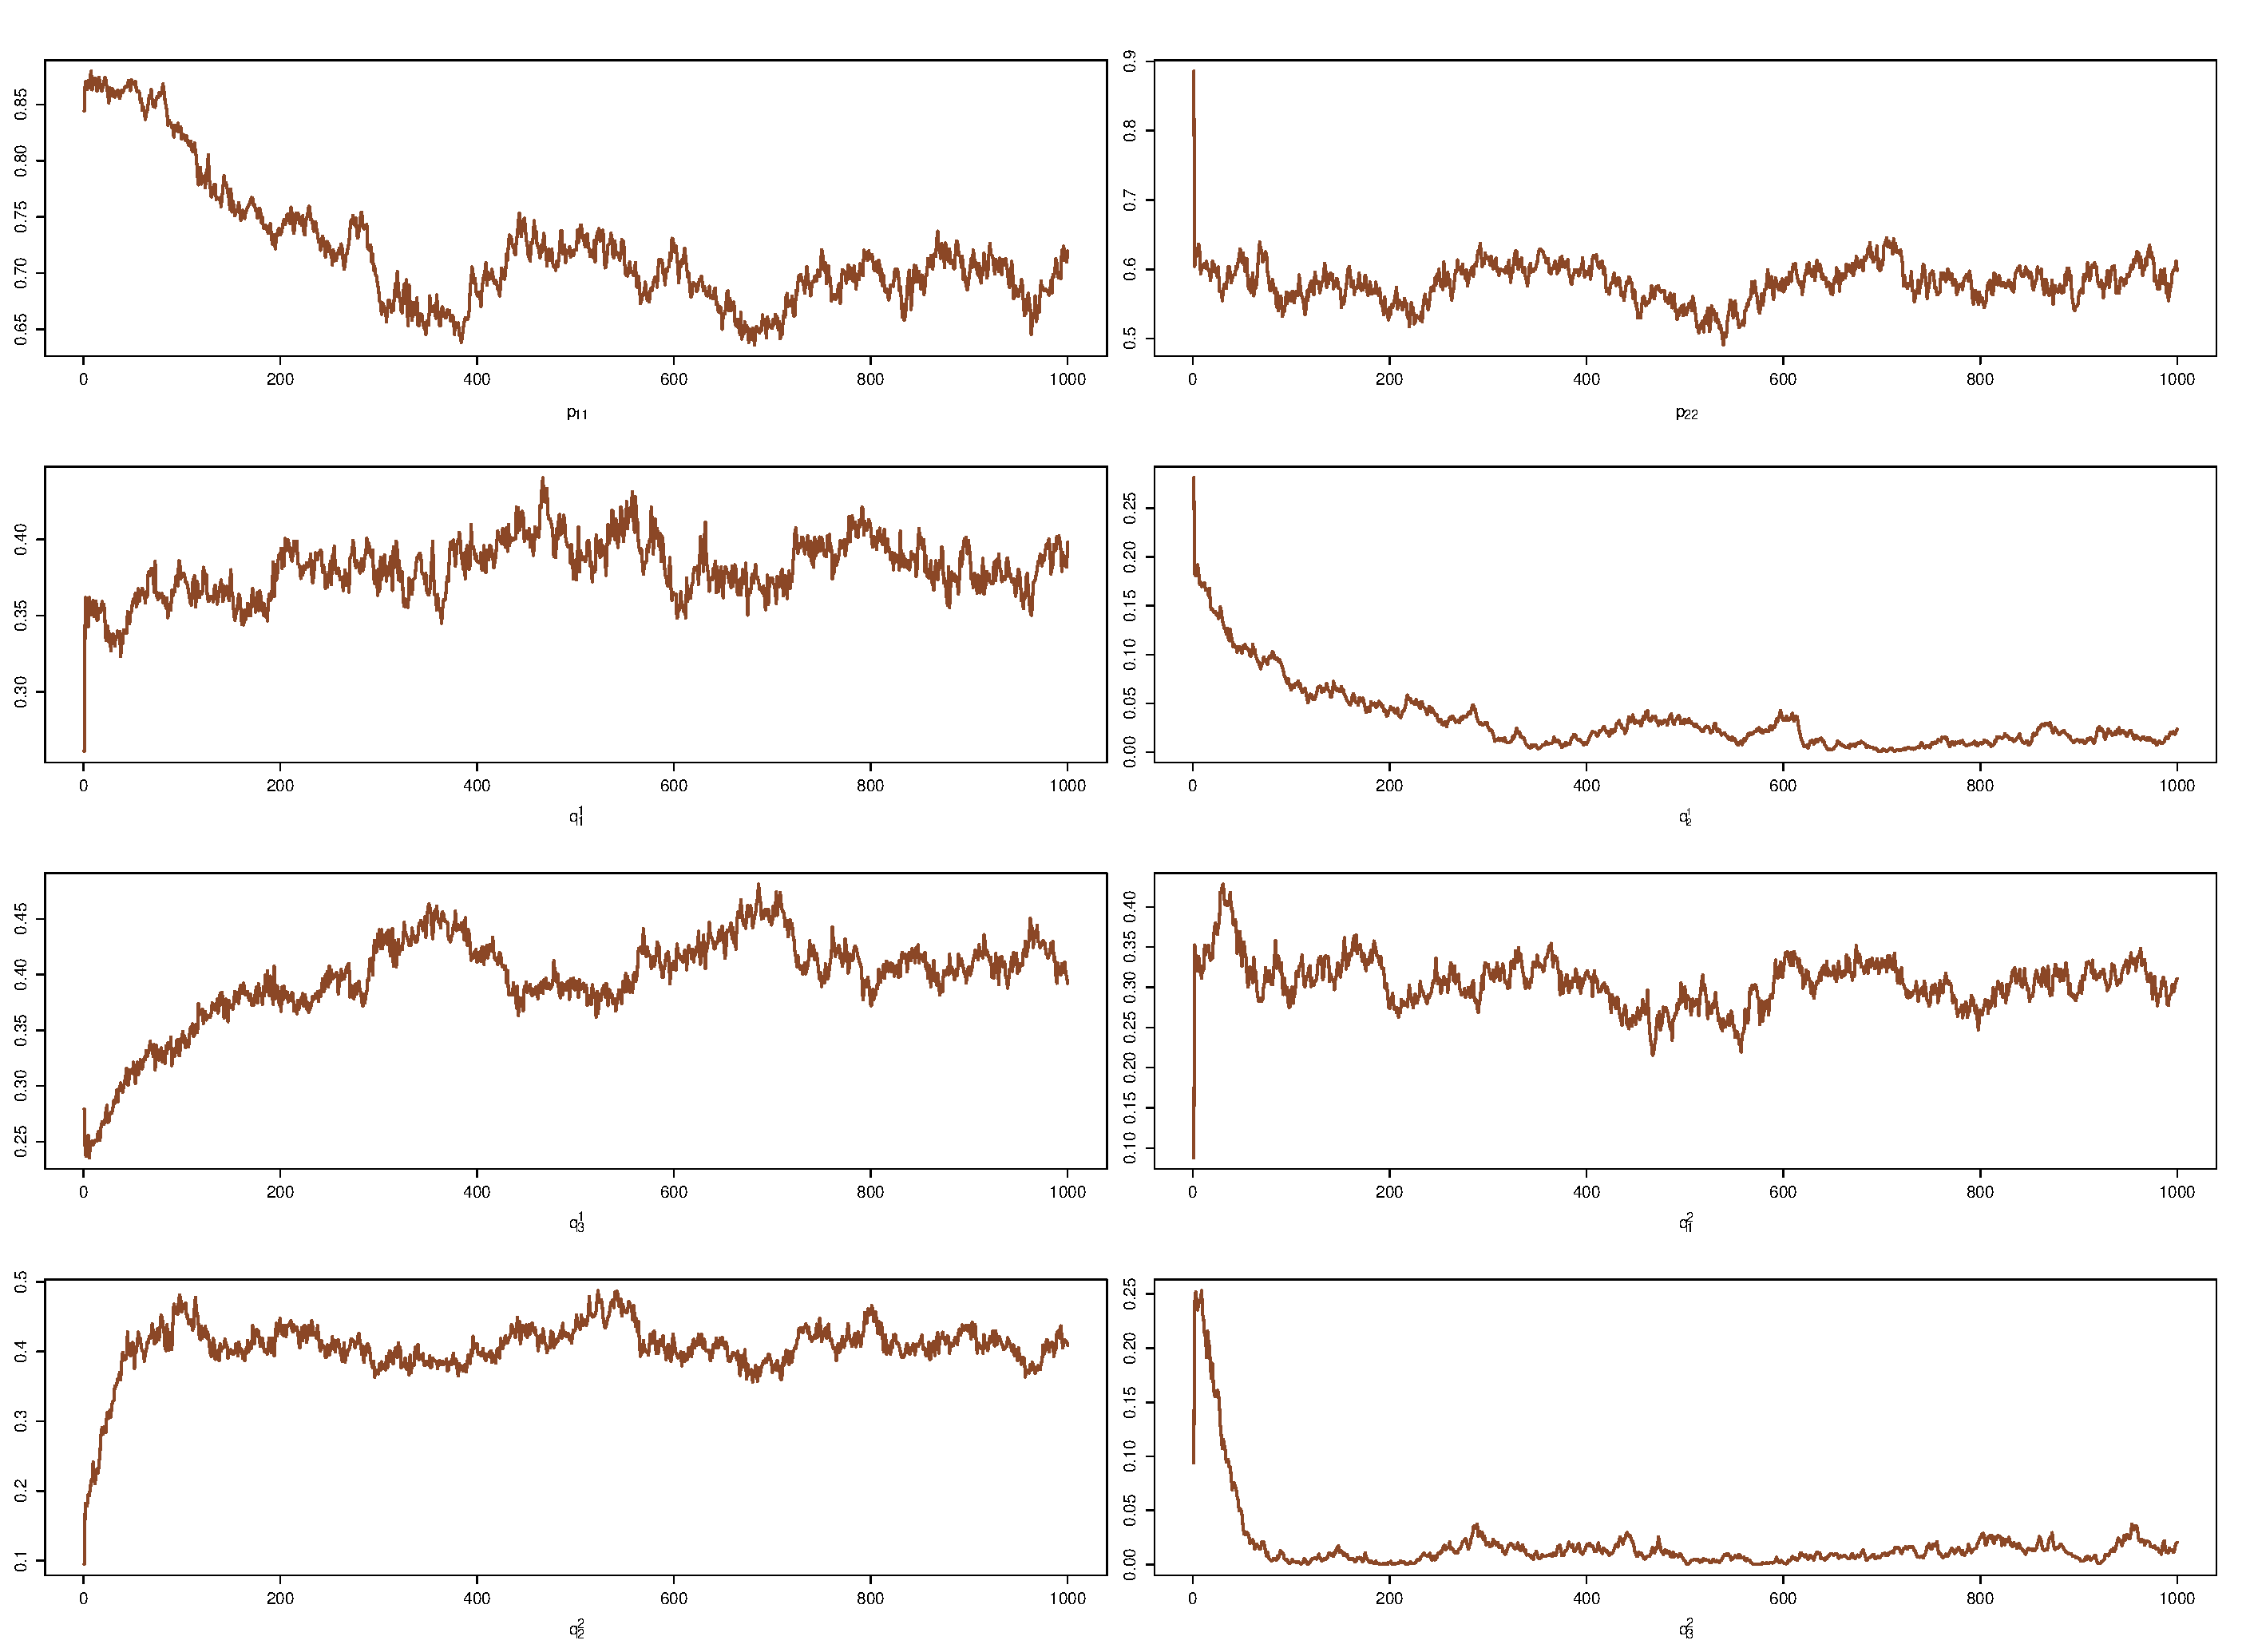
\includegraphics[height=7cm,width=11cm]{figures/GigHmHi.eps}}

\end{slide}\begin{slide}
\slidetitle{Forward-Backward formulae}

Existence of a (magical) recurrence relation that provides the observed
likelihood function in manageable computing time

Called {\em forward-backward} or {\em Baum--Welch} formulas

\end{slide}\begin{slide}
\slidetitle{Observed likelihood computation}

Likelihood of the {\em complete model} simple:
$$
  \ell^c(\btheta|\bx,\by) = \prod_{t=2}^T p_{y_{t-1}y_t}\,f(x_t|\theta_{y_t})
$$
but likelihood of the {\em observed model} is not:
$$
\ell(\btheta|\bx) = \sum_{\by\in\{1,\ldots,\kappa\}^T}  \ell^c(\btheta|\bx,\by) 
$$

\vs\pause
\centerline{\RedOrange{\fbox{\bf \copyright \ ${\mathrm 
O}(\kappa^T)$ complexity}}}

\end{slide}\begin{slide}
\slidetitle{Forward-Backward paradox}

It is possible to express the (observed) likelihood $L^O(\btheta|\bx)$ in 
$$
  \Brown{{\mathrm O}(T^2\times \kappa)}
$$
computations, based on the Markov property of the pair $(x_t,y_t)$.

\hyperlink{Basoo}{\beamergotobutton{Direct to backward smoothing}}

\end{slide}\begin{slide}
\slidetitle{Conditional distributions}

We have
$$
p(\by_{1:t}|\bx_{1:t}) = \frac{f(x_t|y_t)\,p(\by_{1:t}|\bx_{1:(t-1)})}{p(x_t|\bx_{1:(t-1)})}
$$
\emfarite{Smoothing/Bayes}

and
%%\begin{equation}\label{fb2}
$$
p(\by_{1:t}|\bx_{1:(t-1)}) = k(y_t|\by_{t-1})p(\by_{1:(t-1)}|\bx_{1:(t-1)})
$$
\emfarite{Prediction}

where $k(y_t|y_{t-1})=p_{y_{t-1}y_t}$ 
associated with the matrix ${\mathbb P}$ and
$$f(x_t|y_t) = f(x_t|\theta_{y_t})$$

\end{slide}\begin{slide}
\slidetitle{Update of predictive}

Therefore
\begin{eqnarray*}
p(\by_{1:t}|\bx_{1:t}) &=& \frac{p(y_t|\bx_{1:(t-1)})\,f(x_t|y_t)}{p(x_t|\bx_{1:(t-1)})}
\nonumber\\
&=& \frac{f(x_t|y_t)\,k(y_t|\by_{t-1})}{p(x_t|\bx_{1:(t-1)})}
p(\by_{1:(t-1)}|\bx_{1:(t-1)})
\end{eqnarray*}
with the same order of complexity for $p(\by_{1:t}|\bx_{1:t})$ 
as for $p(x_t|\bx_{1:(t-1)})$

\end{slide}\begin{slide}
\slidetitle{Propagation and actualization equations}
$$
p(y_t|\bx_{1:(t-1)}) = \sum_{\by_{1:(t-1)}}\, p(\by_{1:(t-1)}|\bx_{1:(t-1)})\, k(y_t|y_{t-1})
$$
\emfarite{Propagation}

and
$$
p(y_t|x_{1:t}) = \frac{p(y_t|\bx_{1:(t-1)})\,f(x_t|y_t)}{p(x_t|\bx_{1:(t-1)})}\,.
$$
\emfarite{Actualization}

\end{slide}\begin{slide}
\slidetitle{Forward--backward equations (1)}

Evaluation of 
$$
p(y_t | \bx_{1:T}) \quad t \le T
$$
by {\em forward-backward algorithm} 

\pause
Denote $t \le T$
\begin{eqnarray*}
\gamma_t(i) &=& P(y_t = i | x_{1:T}) \\
\alpha_t(i) &=& p(\bx_{1:t}, y_t = i)  \\ 
\beta_t(i) &=& p(\bx_{t+1:T}|y_t=i)
\end{eqnarray*}

\end{slide}\begin{slide}
\slidetitle{Recurrence relations}
Then\small
\[
  {\left\{\begin{array}{lcl}
  \alpha_1(i) & = & f(x_1|y_t = i) \varrho_i\\
  \alpha_{t+1}(j) & = & {\displaystyle f(x_{t+1}|y_{t+1}=j) 
      \sum_{i=1}^{\kappa}\alpha_{t}(i) p_{ij}}\\
  \end{array}\right.}
\]\emfarite{Forward}

\[
  {\left\{\begin{array}{lcl}
  \beta_T(i) & = & 1\\
  \beta_{t}(i) & = & {\displaystyle \sum_{j=1}^{\kappa} p_{ij}} 
  f(x_{t+1}|y_{t+1}=j) \beta_{t+1}(j)\\
  \end{array}\right.}
\]\emfarite{Backward}

and\normalsize
\[
  \label{imos}\BrickRed{
  {\gamma_t(i) = \frac{\alpha_t(i)\beta_t(i)}{\displaystyle 
  \sum_{j=1}^{\kappa} \alpha_t(j)\beta_t(j)}}}
\]

\end{slide}\begin{slide}
\slidetitle{Extension of the recurrence relations}
For
$$
  \xi_t(i,j) = P(y_t =i, y_{t+1} = j|\bx_{1:T}) \qquad i,j=1,\ldots,\kappa,
$$
we also have
$$\BrickRed{
     {\xi_t(i,j) = \frac{\alpha_t(i)\BP_{ij}f(x_{t+1}|y_t=j)
     \beta_{t+1}(j)}{\displaystyle \sum_{i=1}^\kappa\sum_{j=1}^\kappa
     \alpha_t(i)\BP_{ij}f(x_{t+1}|y_{t+1}=j)\beta_{t+1}(j)}}}
$$

\end{slide}\begin{slide}
\slidetitle{Overflows and underflows}

\begin{itemize}\item[$\lightning$]
On-line scalings of the $\alpha_t(i)$'s and $ \beta_T(i) $'s for each $t$ by
$$
  c_t = 1 \Big/ \sum_{i=1}^\kappa \alpha_{t}(i) \quad\hbox{and}\quad
  d_t = 1 \Big/ \sum_{i=1}^\kappa \beta_{t}(i) 
$$
avoid overflows or/and underflows for large datasets
\end{itemize}

\end{slide}\begin{slide}[label=Basoo]
\slidetitle{Backward smoothing}

Recursive derivation of conditionals

We have
$$
p(y_s|y_{s-1},\bx_{1:t})=p(y_s|y_{s-1},\bx_{s:t})
$$
\emfarite{Markov property!}

Therefore $(s=T,T-1,\ldots,1)$
$$
p(y_s|y_{s-1},\bx_{1:T}) \propto k(y_s|y_{s-1})\,f(x_s|y_s)\,
	\sum_{y_{s+1}} p(y_{s+1}|y_s,\bx_{1:T})
$$
\emfarite{Backward equation}

with 
$$
p(y_T|y_{T-1},\bx_{1:T}) \propto k(y_T|y_{T-1}) f(x_T|y_t) \,.
$$

\end{slide}\begin{slide}
\slidetitle{End of the backward smoothing}

The first term is
$$
p(y_1|\bx_{1:t}) \propto \pi(y_1)\,f(x_1|y_1)\,\sum_{y_2} p(y_2|y_1,\bx_{1:t})\,,
$$
with $\pi$ stationary distribution of ${\mathbb P}$\\

\vs\pause
The conditional for $y_s$ needs to be defined for each of the $\kappa$ values of $y_{s-1}$

\centerline{\RedOrange{\fbox{\bf \copyright\ ${\mathrm O}(t\times \kappa^2)$ operations}}}

\end{slide}\begin{slide}
\slidetitle{Details}

Need to introduce unnormalized version of the
conditionals $p(y_t|y_{t-1},\mathbf{x}_{0:T})$ such that
\begin{eqnarray*}
p_T^\star(y_T|y_{T-1},\mathbf{x}_{0:T}) &=& p_{y_{T-1}y_T} f(x_T|y_T)\\
p^\star_{t}(y_t|y_{t-1},\mathbf{x}_{1:T}) &=& p_{y_{t-1}y_t} f(x_t|y_t) 
	\sum_{i=1}^\kappa p^\star_{t+1}(i|y_t,\mathbf{x}_{1:T})\\
p^\star_0(y_0|\mathbf{x}_{0:T}) &=& \varrho_{y_0}\,f(x_0|y_0)\,\sum_{i=1}^\kappa p^\star_1(i|y_0,\mathbf{x}_{0:t})
\end{eqnarray*}

\end{slide}\begin{slide}
\slidetitle{Likelihood computation}

\begin{columns}\column{.55\textwidth}
Bayes formula
\[\Red{
p(\bx_{1:T}) = \frac{p(\bx_{1:T}|\by_{1:T}) p(\by_{1:T})}{p(\by_{1:T}|\bx_{1:T})}
}\]
\column{.4\textwidth}
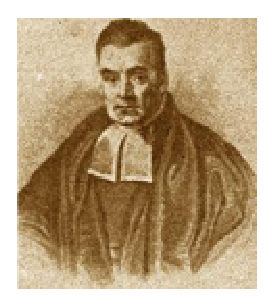
\includegraphics[height=2.5truecm]{figures/TBayes}
\end{columns}
gives a representation of the likelihood based on the
forward--backward formulae and an arbitrary sequence $\bx^o_{1:T}$ (since the
l.h.s.~does {\em not} depend on $\bx_{1:T}$).

\vs\pause
Obtained through the $p^\star_{t}$'s as
$$
p(\mathbf{x}_{0:T}) = \sum_{i=1}^\kappa p^\star_1(i|\mathbf{x}_{0:T})
$$

\end{slide}\begin{slide}
\slidetitle{Prediction filter}

If
$$\Brown{
  \varphi_t(i) = p(y_t =i|\bx_{1:t-1})
}$$

{\RawSienna{\bf Forward equations}}
\begin{eqnarray*}
 \varphi_1(j)  &=& p(y_1 = j) \nonumber\\
 \varphi_{t+1}(j) &=& \frac{1}{c_{t}}\sum_{i=1}^{\kappa} f(x_{t}|y_t=i)
  \varphi_{t}(i) p_{ij} \:\:\: \text{($t \ge 1$)}
\end{eqnarray*}
where
$$
  c_t = \sum_{k=1}^{\kappa} f(x_{t}|y_t=k) \varphi_{t}(k) \,,
$$

\end{slide}\begin{slide}
\slidetitle{Likelihood computation (2)}
Follows the same principle as the backward equations

The (log-)likelihood is thus
\begin{align*}
\log p(\bx_{1:t}) &= 
\sum_{r=1}^{t} \log \left[\sum_{i=1}^{\kappa} 
	p(x_t, y_t = i|\bx_{1:(r-1)})\right] \nonumber\\
&= \sum_{r=1}^{t} \log \left[\sum_{i=1}^{\kappa} f(x_t|y_t=i) \varphi_t(i)\right]
\end{align*}

\end{slide}
\begin{comment}
\subsection{Stochastic volatility}\begin{slide}
\slidetitle{Stochastic volatility}

Simplest stochastic volatility model
$$
  y_t=\beta\exp\left(x_t/2\right)\epsilon_t\,,\qquad \epsilon_t\sim\mathcal{N}(0,1)
$$
with AR$(1)$ log-variance process (or \BrickRed{{\em volatility}}\/)
$$
x_{t+1}=\varphi x_t+\sigma u_t\,,\quad u_t\sim\mathcal{N}(0,1)
$$

\end{slide}\begin{slide}
\slidetitle{First-order difference of AEGON stock}

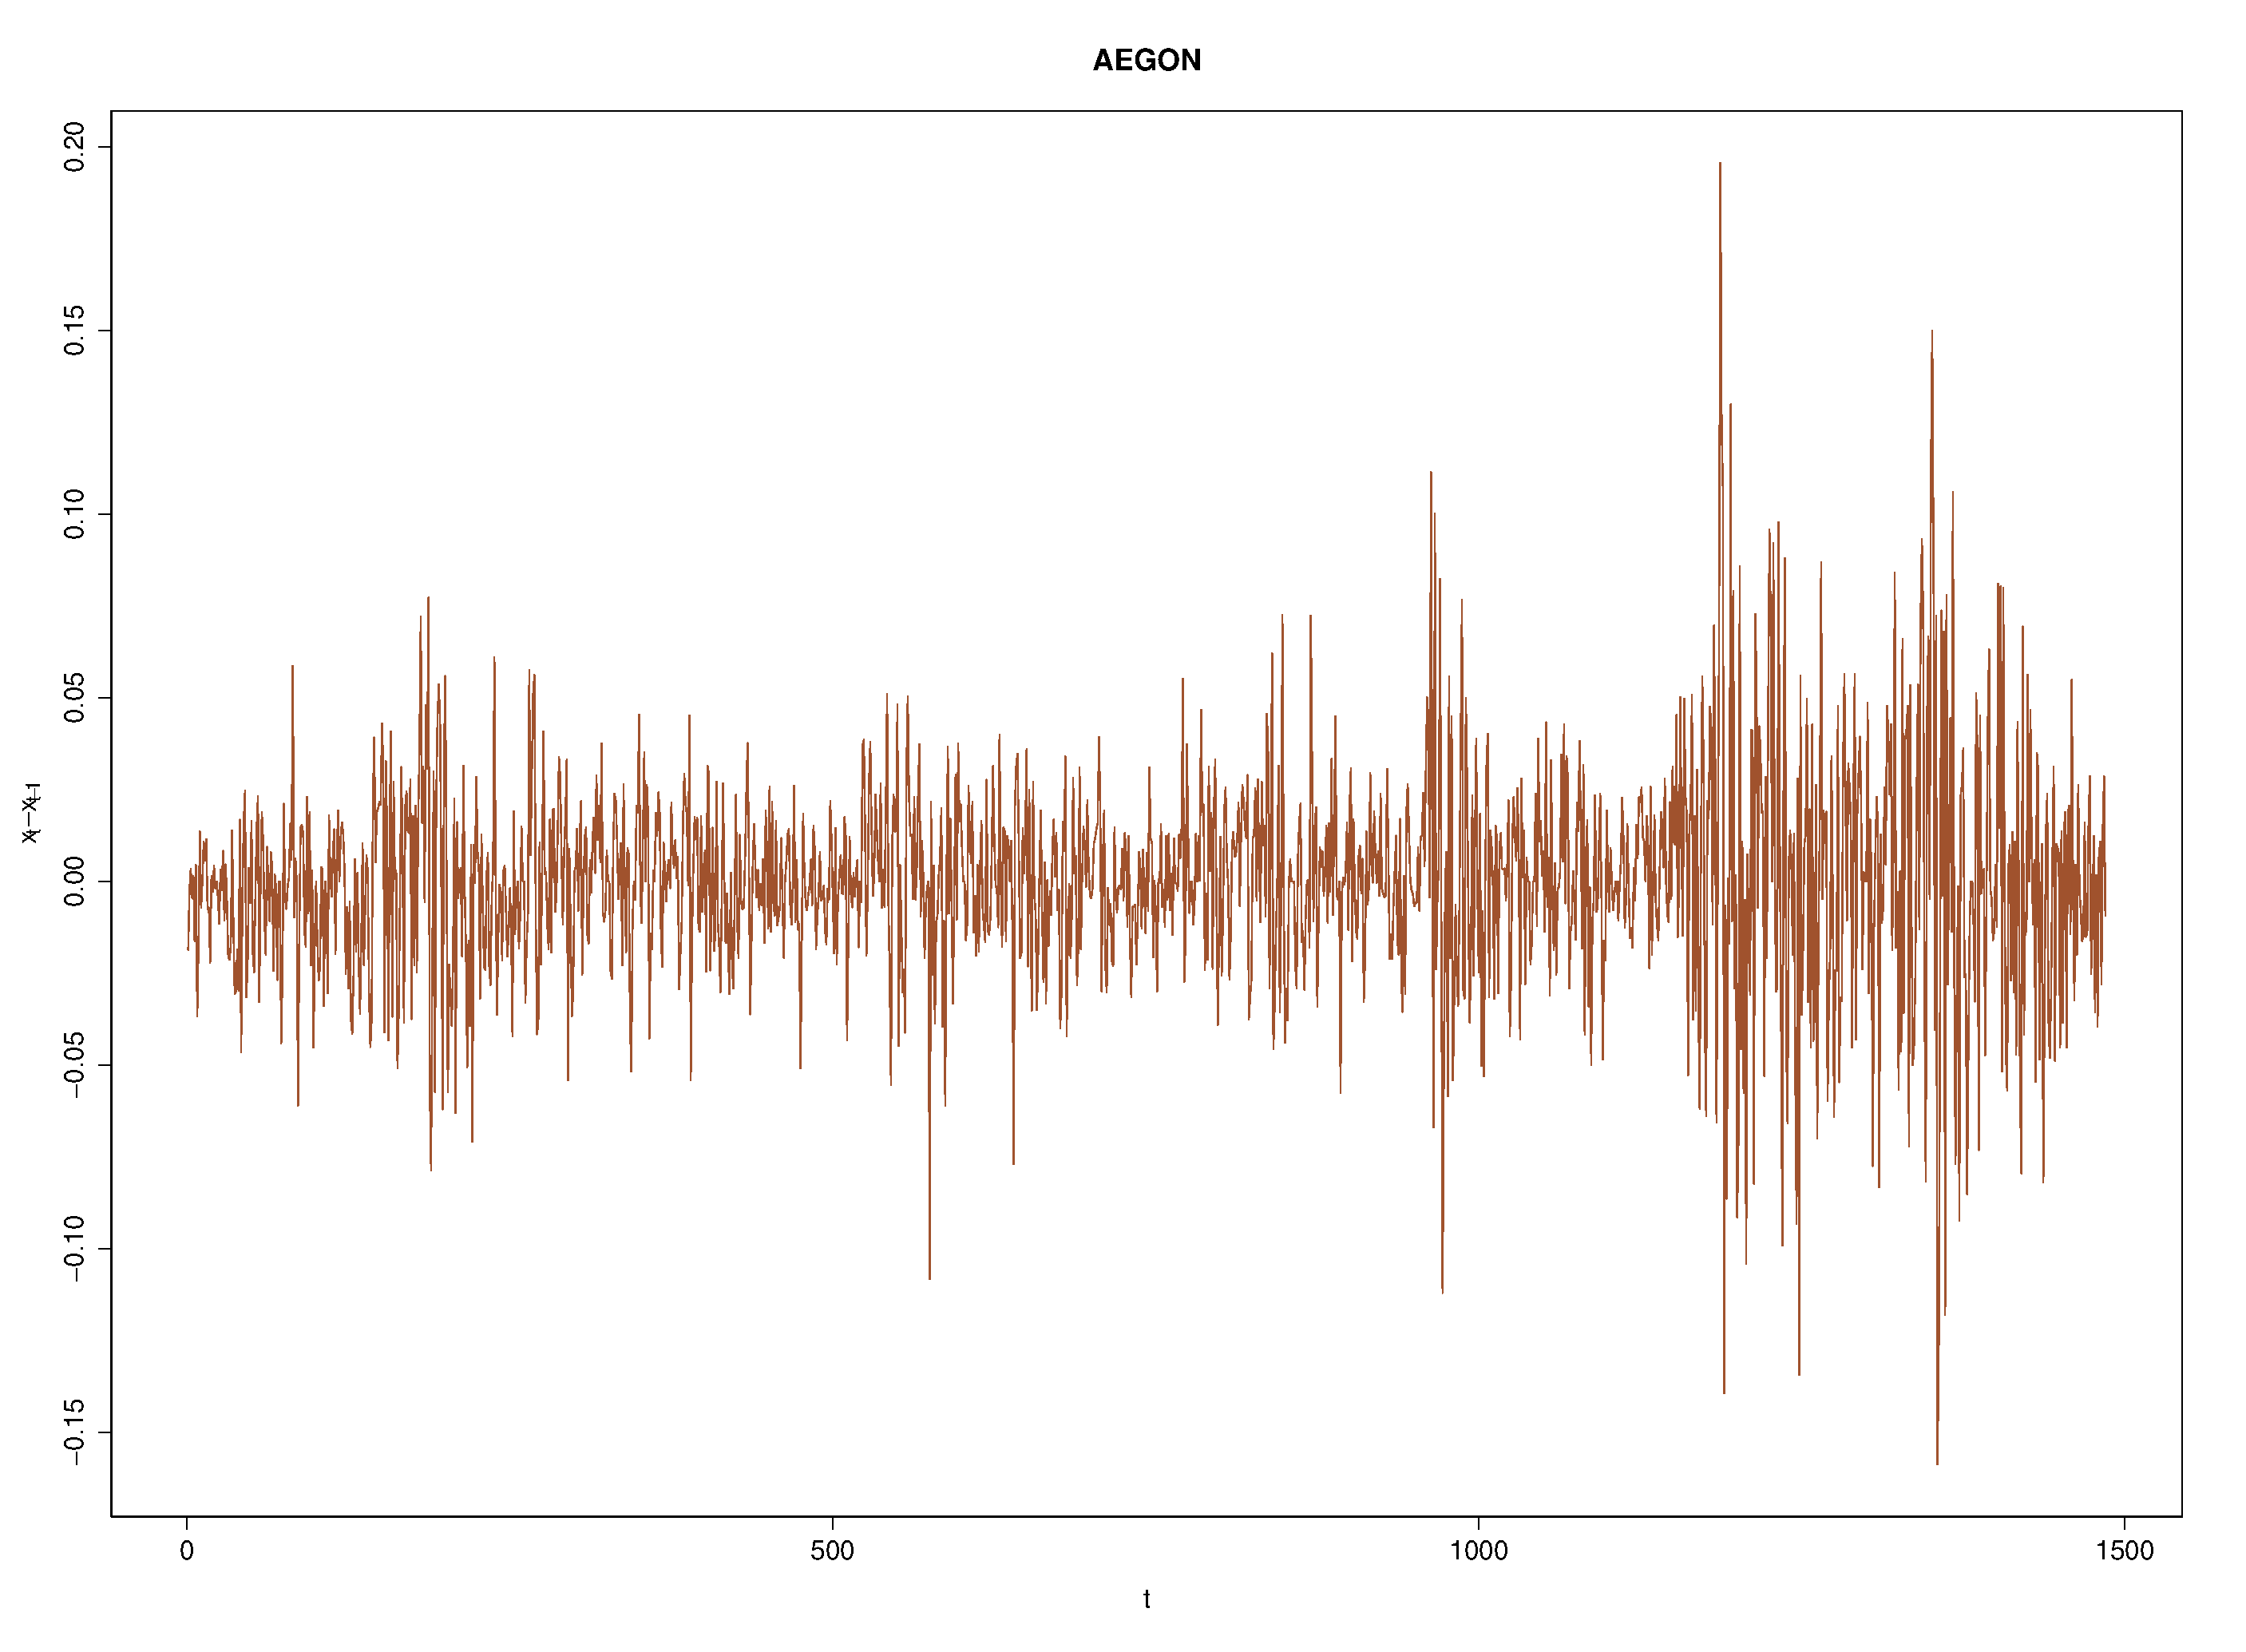
\includegraphics[height=5cm,width=10cm]{figures/aegon.eps}

\end{slide}\begin{slide}
\slidetitle{Completed model}
Observed likelihood unavailable in closed from.

\vs Joint posterior (or conditional) distribution of
the hidden state sequence  $\{x_k\}_{1\le k\le n}$ can be evaluated explicitly 
$$
\prod_{k=2}^K \exp -\left\{ \sigma^{-2} (x_k-\phi x_{k-1})^2 
+ \beta^{-2} \exp(-x_k)y_k^2 +x_k \right\}/2\,,
$$
up to a normalizing constant. 

\vs\pause Volatility often of interest for practitioners

\end{slide}\begin{slide}
\slidetitle{Completion}

Necessary MCMC completion by the missing data $\{x_k\}_{1\le k\le n}$
(same dimension as the data)

\vs\pause
Direct simulation from this distribution impossible because of
\begin{itemize}
\item dependence among the $x_k$'s,
\item dimension of the sequence $\{x_k\}_{1\le k\le n}$, and
\item exponential term $\exp(-x_k)y_k^2$ 
\end{itemize}

\end{slide}\begin{slide}
\slidetitle{Importance sampling}

Natural candidate: replace the exponential term with a quadratic approximation to
preserve Gaussianity.

E.g., expand $\exp(-x_k)$ around its conditional expectation $\phi x_{k-1}$ as 
$$
\exp(-x_k) \approx \exp(-\phi x_{k-1}) \left\{ 1 - (x_k-\phi x_{k-1})
        + \frac{1}{2} (x_k-\phi x_{k-1})^2 \right\}\,.
$$

\end{slide}\begin{slide}
\slidetitle{Importance distribution}

Corresponding Gaussian importance distribution with mean
$$
\mu_k = \frac{\phi x_{k-1}\{ \sigma^{-2}+y_k^2\exp(-\phi x_{k-1})/2 \}
-\{ 1-y_k^2\exp(-\phi x_{k-1}) \}/2}{\sigma^{-2}+y_k^2\exp(-\phi x_{k-1})/2} ,
$$
and variance
$$
\tau^2_k = (\sigma^{-2}+y_k^2\exp(-\phi x_{k-1})/2)^{-1}\,.
$$

Prior proposal on $x_1$, $x_1\sim\mathcal{N}(0,\sigma^2)$.

\end{slide}\begin{slide}
\slidetitle{Importance weights}

Simulation starts with $x_1$ and proceeds forward to $x_n$, 
each $x_k$ being generated conditional on $y_k$ and 
the previously generated $x_{k-1}$.

Importance weight computed sequentially as the product of
$$
\frac{
  \exp -\left\{ \sigma^{-2} (x_k-\phi x_{k-1})^2 + \exp(-x_k)y_k^2 +x_k \right\}/2
}{
  \exp -\left\{ \tau^{-2}_k (x_k-\mu_k)^2 \right\} \tau_k^{-1}
} \,.
$$

\end{slide}\begin{slide}
\slidetitle{Poor output}

Results quite variable but not very encouraging: 
For small series, simulated $\{x_k\}_{1\le k\le n}$ most often unrelated 
to the simulated volatility.

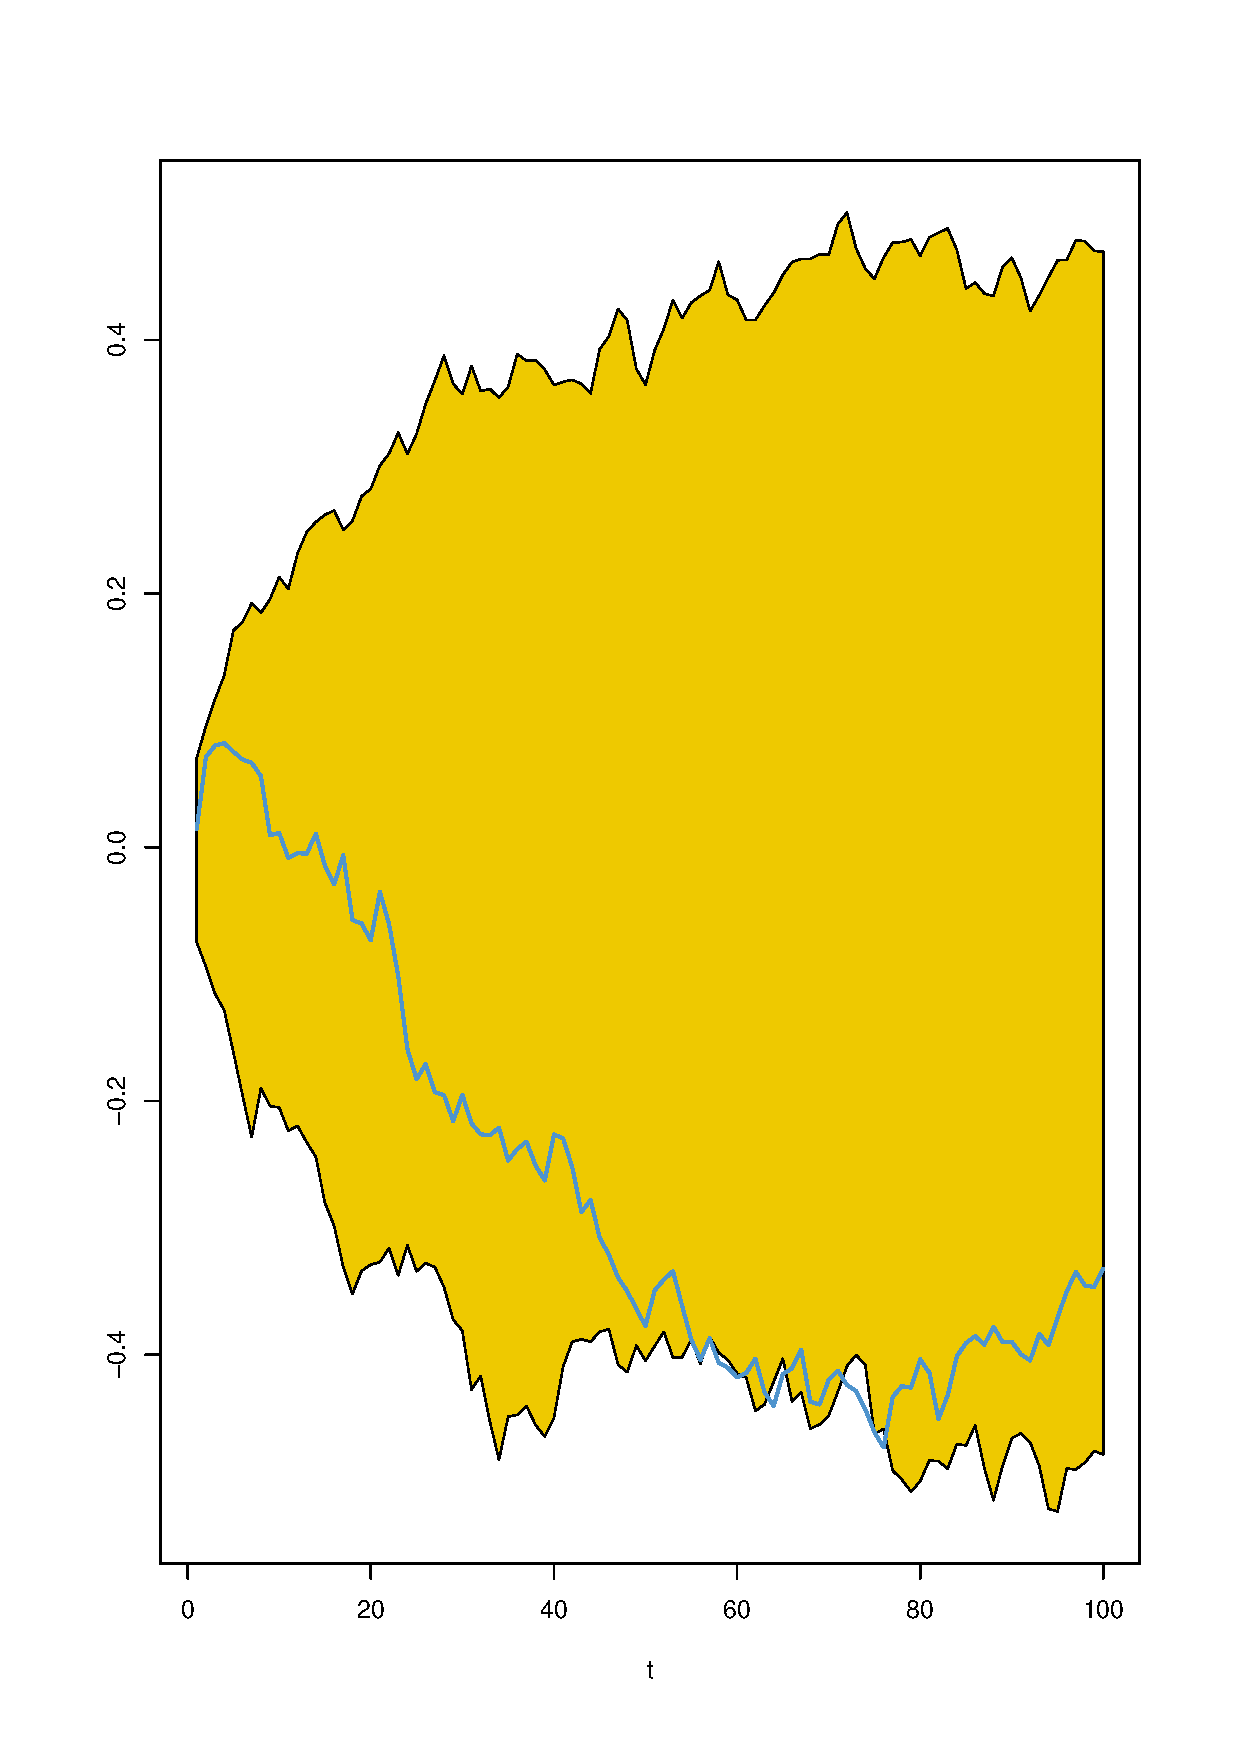
\includegraphics[width=10cm,height=5cm]{figures/stovol2}
\noindent{Range of simulated $\{x_k\}_{1\le k\le 100}$,
compared with true value.}

\end{slide}\begin{slide}
\slidetitle{Curse of dimensionality}
Illustration of the difficulty in selecting a ``good importance distribution": \\

Importance functions that agree with the target
distribution $\mu$ are increasingly difficult to find as the dimension
grows and usually proves impossible for large dimension problems.

\end{slide}\end{document}\begin{slide}
\slidetitle{Slice alternative}

Simulation from
$$
\pi(x) \propto \exp - \left\{ \sigma^2(x-\mu)^2 + \beta^2 \exp(-x)y^2 + x \right\}/2\,,
$$
simplified in 
$$
\exp - \left\{ x^2 + \alpha \exp(-x) \right\}
$$
wlog.

Slice sampling means simulating from a uniform distribution on 
$$
\mathfrak{A} = 
\left\{x; \exp - \left\{ x^2 + \alpha \exp(-x) \right\} / 2 \ge u \right\}
= \left\{x; x^2 + \alpha \exp(-x) \le \omega \right\}
$$
if $\omega = -2 \log u$. 

\end{slide}\begin{slide}
While inversion of 
$$
x^2 + \alpha \exp(-x)=\omega
$$
impossible analytically, 
\begin{itemize}
\item the function is convex ($\alpha>0$) and 
\item previous value of $x$ belong to $\mathfrak{A}$ 
\end{itemize}
thus possible to solve this equation by trial-and-error. 

No need to solve exactly this equation: an interval that contains 
$\mathfrak{A}$ is sufficient to simulate from the uniform distribution 
on $\mathfrak{A}$.

\end{slide}\begin{slide}
\includegraphics[height=7cm,width=\textwidth]{/home/xian/Talks/Oulu/figures/stosli}
\centerline{$\alpha=2$}

\end{slide}\begin{slide}
Simulation of the whole volatility sequence by a step-by-step Gibbs algorithm:\\
\colorbox{LightGrey}{\makebox[0.9\textwidth][c]{\parbox{0.85\textwidth}{{\sf
\Brown{
\noindent For $t=1,\dots,T$, do
\begin{itemize}
\item[] For $k=0,\dots,n$,
\begin{enumerate}
\item Simulate 
\begin{align*}
u_k \sim\hbox{U}\bigg(0,\exp -&\left\{ \sigma^{-2}(x_k-\phi x_{k-1})^2 
+ \sigma^{-2}(x_{k+1}-\phi x_k)^2\right.\\
&\left.+ \beta^2 \exp(-x_k)y_k^2 + x_k \right\}/2\ \big)
\end{align*}
\item Simulate $x_k\sim\hbox{U}(A_k)$  where
\begin{align*}
A_k = \big\{x;\,\exp - &\left\{ \sigma^{-2}(x_k-\phi x_{k-1})^2 
+ \sigma^{-2}(x_{k+1}-\phi x_k)^2 \right.\\
&\left.+ \beta^2 \exp(-x_k)y_k^2 + x_k \right\}/2\,\ge u_k\big\}
\end{align*}
\end{enumerate}
\end{itemize}
}}}}}

(We omit the obvious corrections at the endpoints of the sequence $\bx_{0:n}$.)

\end{slide}\begin{slide}
But lauching this algorithm does not produce any satisfactory result
because of the slice sampler:\\ when solving 
$$
\sigma^{-2}(x_k-\phi x_{k-1})^2 
+ \sigma^{-2}(x_{k+1}-\phi x_k)^2 + \beta^2 \exp(-x_k)y_k^2 + x_k = \omega_k
$$
some values of the parameters $\beta$, $x_{k-1}$, $x_{k-1}$, and $y_k$ 
lead to numerical difficulties that cause the algorithm to stop.

\end{slide}\begin{slide}
\slidetitle{Slice sampling (2)}
Separate the target distribution
\begin{align*}
\varphi^{k}(x|x_{k-1},x_{k+1},y_k) &\propto \exp - \left\{ \sigma^{-2}(x_k-\phi x_{k-1})^2 
+ \sigma^{-2}(x_{k+1}-\phi x_k)^2 \right.\\
&\left.+ \beta^2 \exp(-x_k)y_k^2 + x_k \right\}/2
\end{align*}
as
$$
\varphi^{k}(x_k|x_{k-1},x_{k+1},y_k) \propto  \exp - (x_k-\mu_k)^2\tilde\sigma^{-2}\,
\int_0^{\exp\{-\beta^2 \exp(-x_k)y_k^2/2\}} \,\hbox{d}u_k
$$
where
$$
\mu_k = \frac{\sigma^{-2}\phi(x_{k-1}+x_{k+1})-.5}{\sigma^{-2}(1+\phi^2)}
\qquad\hbox{and}\qquad \tilde\sigma^{-2}= \sigma^{-2}(1+\phi^2)
$$

Joint density proportional to
$$
\exp - (x_k-\mu_k)^2\tilde\sigma^{-2}\,
\mathbb{I}_{[0,\exp\{-\beta^2 \exp(-x_k)y_k^2/2\}]}(u_k)\,.
$$

\end{slide}\begin{slide}
Algorithm  modified in
\colorbox{LightGrey}{\makebox[0.9\textwidth][c]{\parbox{0.85\textwidth}{{\sf
\Brown{
\noindent For $t=1,\dots,T$, do
\begin{itemize}
\item[] For $k=0,\dots,n$,
\begin{enumerate}
\item Simulate
$$
u_k \sim\hbox{U}\bigg(0,\exp - \left\{\beta^2 \exp(-x_k)y_k^2 + x_k \right\}/2\ \bigg)
$$
\item Simulate $x_k$ from a normal $\mathcal{N}(\mu_k,\tilde\sigma^2)$ distribution restricted to
$$
B_k = \left(-\log \left[-2\log \left\{ u_k/\beta^2 y_k^2 \right\} \right] , \infty \right)
$$
\end{enumerate}
\end{itemize}
}}}}}

\includegraphics[height=5cm,width=12cm]{/home/xian/Talks/Oulu/figures/stogib}
\vskip -.3truecm
\noindent{\label{fig:stogib}Gibbs sampling simulation for a simulated sequence of $2500$ points
and $500$ iterations ($\phi=.99$, $\beta=.07$ and
$\sigma=.01$). Full graph is the truth and the dotted curve
is the simulated sequence after $500$ iterations. The range corresponds to the $500$
iterations, started at the true volatility sequence.}

\includegraphics[height=5cm,width=11cm]{/home/xian/Talks/Oulu/figures/stogib0}
\vskip -.3truecm
\noindent{\label{fig:stogib0}Same thing when the volatility 
is started at $0$, for $1,500$ points and $5,000$ iterations. The range is based on the last
$500$ iterations.}

\includegraphics[height=11cm,width=8cm,angle=270]{/home/xian/Talks/Oulu/figures/stogibT}
\vskip -.3truecm
\noindent{\label{fig:stogibT}Comparison of the initialization effect when
initialized {\em (top)} at the true value and {\em (bottom)} at $0$, after $25,000$ 
iterations (range based on the last $500$ iterations).}

\end{slide}\begin{slide}
\slidetitle{General MCMC algorithm}
\OrangeRed{{\bf Lack of robustness:}}\\ the MCMC algorithm
may fail to converge for long series or extreme values of the parameters 
$\beta$ and $\varphi$.

Very sensitive to the generation of the missing data 

May well fail to converge even when initialized at the true parameter values.

\end{slide}\begin{slide}
\slidetitle{Parameter simulation (1)}
Posterior distributions for $\beta^2$ and $\sigma^2$  conditional on the $x_t$'s
and $z_t$'s both inverse Gamma distributions with $(n-1)/2$ shape parameters and
$$
\sum_{t=1}^ny_t^2\exp(-z_t)/2\quad\hbox{ and }\quad
\sum_{t=2}^n\left(z_t-\varphi z_{t-1}\right)^2/2
$$
scales 

\end{slide}\begin{slide}
\slidetitle{Parameter simulation (2)}
Conditional distribution of $\varphi$ proportional to
$$
\sqrt{1-\varphi^2}
\exp-\left(\varphi^2\sum_{t=2}^{n-1}z_t^2-2\varphi\sum_{t=2}^nz_tz_{t-1}\right)\big/{2\sigma^2}
\,\mathbb{I}_{]-1,1[}(\varphi)\,,
$$
and standard proposal truncated normal on $]-1,1[$ with mean and variance
$$
{\sum_{t=2}^nz_tz_{t-1}}\Big/{\sum_{t=2}^{n-1}z_t^2}\quad\hbox{and}\quad
{\sigma^2}\Big/{\sum_{t=2}^{n-1}z_t^2}
$$

\end{slide}\begin{slide}
\slidetitle{Missing data simulation(2)}
Simulation of $z_t|y,\varphi,\sigma^2$ $(2\le t\le n-1)$, proportional to
$$
\exp\left\{ -0.5\left(1+\varphi^2\right)\left(z_t-\mu_t\right)^2/\sigma^2-0.5
\exp\left(-z_t\right)y_t^2/\beta^2-0.5z_t \right\}\,,
$$
where $\mu_t=\varphi\left(z_{t-1}+z_{t+1}\right)/(1+\varphi^2)$. 

\end{slide}\begin{slide}
\MidnightBlue{{\bf Solution:}}\\
Expand $\exp\left(-z_t\right)$ by a Taylor expansion around
$\mu_t$. 

Normal proposal with mean
$$
\frac{\left(1+\varphi^2\right)\mu_t/\sigma^2+0.5\exp\left(-\mu_t\right)y_t^2
\left(1+\mu_t\right)/\beta^2-0.5} {\left(1+\varphi^2\right)/\sigma^2
+0.5\exp\left(-\mu_t\right)y_t^2/\beta^2}
$$
and variance
$$
1\big/{\left\{ \left(1+\varphi^2\right)/\sigma^2+0.5\exp\left(-\mu_t\right)y_t^2/\beta^2\right\}}\,.
$$

\begin{center}
\includegraphics[height=6cm,width=10cm]{/home/xian/Papers/CMR03/datas.eps}
\noindent{Weekly {\em (upper)} and daily {\em (lower)} simulated datasets with $n=1000$
observations $y_t$ {\em (black)} and volatilities $z_t$ {\em (red)}.}
\label{fig:datas}
\end{center}

\end{slide}\begin{slide}
\begin{center}
\includegraphics[height=6cm,width=10cm]{/home/xian/Papers/CMR03/hmdata1.eps}
\noindent{Weekly dataset: evolution of the MCMC samples for the three parameters {\em (left)}
and convergence of the MCMC estimators {\em (right)}.}
\label{fig:hmdata1}
\end{center}

\end{slide}\begin{slide}
\begin{center}
\includegraphics[height=6cm,width=10cm]{/home/xian/Papers/CMR03/hmredata1.eps}
\noindent{Weekly dataset: estimation of the stochastic volatility (in black the true volatility
and in red the MCMC estimation based on the last 5000 iterations).}
\label{fig:hmredata1}
\end{center}

\end{slide}\begin{slide}
\begin{center}
\includegraphics[height=6cm,width=10cm]{/home/xian/Papers/CMR03/hmdata2.eps}
\centerline{Daily dataset: same legend as Figure \ref{fig:hmdata1}.}
\end{center}

\end{slide}\begin{slide}
\begin{center}
\includegraphics[height=6cm,width=10cm]{/home/xian/Papers/CMR03/hmredata2.eps}
\centerline{Daily dataset: same legend as Figure \ref{fig:hmredata1}.}
\end{center}

\end{slide}\begin{slide}
\slidetitle{Population Monte Carlo}
\markboth{{\sf \Gray{AR(p)/MA(q)}/\Red{Sto'vol:PMC}}}{{\sf \Gray{AR(p)/MA(q)}/\Red{Sto'vol:PMC}}}

{\BrickRed{\bf A dynamic extension to importance sampling}}

As in MCMC algorithms, introduction of a
\RedOrange{{\em temporal dimension}} :
$$
x_i^{\Red{(t)}} \sim q_{\Red{t}}(x|x_i^{\Red{(t-1)}}) \qquad i=1,\ldots,n,\quad t=1,\ldots
$$
and
$$
\hat{\mathfrak{I}}_t = \frac{1}{n}\,\sum_{i=1}^n \varrho_i^{(t)} h(x_i^{(t)})
$$
is still unbiased for
$$
\varrho_i^{(t)} = \frac{\pi(x_i^{(t)})}{q_{t}(x_i^{(t)}|x_i^{(t-1)})}\,, \qquad i=1,\ldots,n
$$

\end{slide}\begin{slide}
\MidnightBlue{{\bf Reason why:}}
\begin{align*}
\mathbb{E} \bigg[ h(x^{(t)}) &\, \left. \frac{\pi(x^{(t)})}{q_{t}(x^{(t)}|x^{(t-1)})} \right] \\
&=\ \int h(x)\,\frac{\pi(x)}{q_{t}(x|y)}\,q_{t}(x|y)\,g(y)\,\hbox{d}x\,\hbox{d}y  \\
&=\ \int h(x)\,\pi(x) \,\hbox{d}x 
\end{align*}
for \Red{{\bf any distribution}} $g$ on $x^{(t-1)}$

\end{slide}\begin{slide}
{\BrickRed{\bf Variance decomposition}}

Furthermore,
$$
\varm\left( \hat{\mathfrak{I}}_t \right) =  \frac{1}{n^2}\ \sum_{i=1}^n 
\varm\left(\varrho_i^{(t)} h(x_i^{(t)})\right) \,,
$$
if $\varm\left(\varrho_i^{(t)}\right)$ exists, because the $x_i^{(t)}$'s
are conditionally uncorrelated

\Brown{{\bf Note: }} Decomposition still valid for correlated $x_i^{(t)}$'s
when incorporating weights $\varrho_i^{(t)}$

\end{slide}\begin{slide}
\BrickRed{{\bf Normalising constants}}

In general, $\pi$ is unscaled and 
$$
\varrho_i^{(t)} \propto \frac{\pi(x_i^{(t)})}{q_{it}(x_i^{(t)})}\,,
\qquad i=1,\ldots,n\,,
$$
scaled so that 
$$
\sum_i \varrho_i^{(t)} = 1
$$

\end{slide}\begin{slide}
\begin{itemize}
\item Loss of the unbiasedness property and the variance decomposition
\item Normalising constant can be estimated by
$$
\varpi_t =
\frac{1}{tn}\,\sum_{\tau=1}^t\,\sum_{i=1}^n\,
\frac{\pi(x_i^{(\tau)})}{q_{i\tau}(x_i^{(\tau)})}
$$
\item Variance decomposition (approximately) recovered if $\varpi_{t-1}$ used instead
\end{itemize}

\end{slide}\begin{slide}
\BrickRed{{\bf Resampling}}

Over iterations (in $t$), weights may {\em degenerate}:\\ e.g.,
$\varrho_1\equiv 1$, while $\varrho_2,\ldots,\varrho_n$ negligible 

Use instead Rubin's (1987) \RedOrange{{\em systematic resampling:}} at each iteration
resample the $x_i^{(t)}$'s according to their weight $\varrho_i^{(t)}$ and reset the weights
to $1$ \Maroon{(preserves ``unbiasedness"/increases variance)}

\end{slide}\begin{slide}

\baro
\centerline{\Brown{{\bf PMCA: Population Monte Carlo Algorithm}}}
\smallskip\hrule height.2pt\smallskip
\colorbox{LightGrey}{\makebox[0.95\textwidth][c]{\parbox{0.95\textwidth}{
{\sffamily
\noindent For $t=1,\ldots,T$
\begin{enumerate}
\item[ ] For $i=1,\ldots,n$,
\begin{enumerate}
\item\label{zistep} Select the generating distribution $q_{it}(\cdot)$
\item Generate $x_i^{(t)}\sim q_{it}(x)$
\item Compute $\varrho_i^{(t)} = \pi(x_i^{(t)})/q_{it}(x_i^{(t)})$
\end{enumerate}
\item[ ] Normalise the $\varrho_i^{(t)}$'s to sum up to $1$
\item[ ] Resample $n$ values from the $x_i^{(t)}$'s with replacement,
using the weights $\varrho_i^{(t)}$, to create the sample $(x_1^{(t)},\ldots,x_n^{(t)})$
\end{enumerate}
}}}}
\barba

\end{slide}\begin{slide}
\slidetitle{Back to mixtures of distributions}

Observation of an iid sample $\bx=\left(x_1,\ldots,x_n\right)$ from
$$
p{\cal N}(\mu_1,\sigma^2) + (1-p){\cal N}(\mu_2,\sigma^2),
$$
with $p\ne 1/2$ and $\sigma>0$ known.

Usual ${\cal N}(\theta,\sigma^2/\lambda)$ prior on $\mu_1$ and $\mu_2$:
$$
\pi(\mu_1,\mu_2|\bx) \propto f(\bx|\mu_1,\mu_2) \, \pi(\mu_1,\mu_2)
$$

\end{slide}\begin{slide}
{\BrickRed{\bf Population Monte Carlo Algorithm}}\\
\baro
\colorbox{LightGrey}{\makebox[0.99\textwidth][c]{\parbox{0.95\textwidth}{
{\sffamily
\noindent {\bf Step $0$: Initialisation}
\begin{itemize}
\item[] For $j = 1,\ldots,n=pm$, choose $\left(\mu_1\right)_j^{(0)},\left(\mu_2\right)_j^{(0)}$
\item[] For $k = 1,\ldots,p$, set $r_k=m$
\end{itemize}
\noindent {\bf Step $i$: Update $(i=1,\ldots,I)$}
\begin{itemize}
\item[ ] For $k = 1,\ldots,p$,
\begin{enumerate}
\item generate a sample of size $r_k$ as
$$
\left(\mu_1\right)_j^{(i)}\sim\mathcal{N}\left(\left(\mu_1\right)_j^{(i-1)},v_k\right)
\quad\mbox{and}\quad 
\left(\mu_2\right)_j^{(i)}\sim\mathcal{N}\left(\left(\mu_2\right)_j^{(i-1)},v_k\right)
$$
\end{enumerate}
\end{itemize}
}}}}\\

\colorbox{LightGrey}{\makebox[0.95\textwidth][c]{\parbox{0.95\textwidth}{
{\sffamily
\begin{itemize}
\item[ ] \begin{itemize}
\item[2.] compute the weights
$$\varrho_j\propto\frac{f\left(\bx\big|\left(\mu_1\right)_j^{(i)},\left(\mu_2\right)_j^{(i)}\right)
\pi\left(\left(\mu_1\right)_j^{(i)},\left(\mu_2\right)_j^{(i)}\right)}
{\varphi\left(\left(\mu_1\right)_j^{(i)}\big|\left(\mu_1\right)_j^{(i-1)},v_k\right)
\varphi\left(\left(\mu_2\right)_j^{(i)}\big|\left(\mu_2\right)_j^{(i-1)},v_k\right)}$$
\end{itemize}
\item[ ] Resample the
$\left(\left(\mu_1\right)_j^{(i)},\left(\mu_2\right)_j^{(i)}\right)_j$ using the
weights $\varrho_j$,
\item[ ] For $k = 1,\ldots,p$, 
\begin{itemize}
\item[] update $r_k$ as the number of elements generated with variance 
$v_k$ which have been resampled.
\end{itemize}
\end{itemize}
}}}}
\barba

\end{slide}\begin{slide}
\PineGreen{{\bf Details}}\\
After an arbitrary initialisation, use of the previous (importance) sample
(after resampling) to build random walk proposals, 
$$
\mathcal{N}(
\left(\mu\right)_j^{(i-1)},v_j)
\eqno{\BrickRed{[=q_{ji}]}\quad\qquad}
$$
with a multiscale variance $v_j$
within a predetermined set of $p$ scales
ranging from $10^3$ down to $10^{-3}$, whose importance is proportional
to its survival rate in the resampling step.

\MidnightBlue{{\bf Rao--Blackwellisation}} over choice of $v_k$ is possible
and reduces variance \emfarite{Celeux, Marin \&\ Robert, 2003}

\end{slide}\begin{slide}
\begin{center}
\centerline{\quad\psfig{figure=/home/xian/Papers/CMR03/pmc2mix.eps,height=5.5cm,width=12cm}}
\noindent{Representation of the log-posterior distribution via {\sf R image} and {\sf contours}
procedures with the Rao--Blackwellised PMC weighted sample after 30 iterations 
(the weights are proportional to the circles at each point).}
\label{fig:pmc2mix}
\end{center}

\end{slide}\begin{slide}
\slidetitle{Comparison with Gibbs sampling}
\begin{itemize}
\item Based on completion of data by allocations \emfarite{EM algorithm}
\item Single chain of $(\mu_1,\mu_2)$'s
\item Sensitivity to initial values may jeopardize convergence
\item Attraction to local mode like EM algorithm
\end{itemize}

\end{slide}\begin{slide}
\begin{center}
\centerline{\quad\psfig{figure=/home/xian/Papers/CMR03/hmmix.eps,height=5.5cm,width=12cm}}
\centerline{Same graph for the last 1000 points of 10,000 iterations of a Gibbs sampler.
}
\end{center}

\end{slide}\begin{slide}
\slidetitle{Back to SV models}
Run a PMC sampler with exactly the same proposals as completion MCMC

\RawSienna{{\bf Results:}}\\
Better parameter estimates {\em and} volatility reconstruction for PMC than
for MCMC

\end{slide}\begin{slide}
\begin{center}
\includegraphics[height=6cm,width=10cm]{/home/xian/Papers/CMR03/pmcdata1.eps}
\noindent{Weekly dataset: evolution over iterations of the Rao--Blackwellised PMC approximation
{\em (left)} and 10th iteration weighted PMC sample {\em (right)}.}
\label{fig:pmcdata1}
\end{center}

\end{slide}\begin{slide}
\begin{center}
\includegraphics[height=6cm,width=10cm]{/home/xian/Papers/CMR03/pmcredata1.eps}
\noindent{Weekly dataset: estimation of the stochastic volatility (in black the true volatility
and in red the PMC estimation based on the 10th iteration weighted PMC sample).}
\label{fig:pmcredata1}
\end{center}

\end{slide}\begin{slide}
\begin{center}
\includegraphics[height=6cm,width=10cm]{/home/xian/Papers/CMR03/pmcdata2.eps}
\centerline{Daily dataset: same legend as Figure \ref{fig:pmcdata1}..}
\end{center}

\end{slide}\begin{slide}
\begin{center}
\includegraphics[height=6cm,width=10cm]{/home/xian/Papers/CMR03/pmcredata2.eps}
\centerline{Daily dataset: same legend as Figure \ref{fig:pmcredata1}.}
\end{center}

\end{slide}
\end{comment}
